\section{Research Design and Preliminary Results}
Following explains the plans to accomplish the specific aims outlined in section \ref{section:Introduction}. Also, the preliminary results related to each section come afterward.

\subsection{Aim 1: Enhance multi-spectral tissue classification by incorporating multiple modalities with different spatial resolutions}
\label{section:Aim1ResearchDesign}

\subsubsection{Introduction}
\label{section:Aim1Intro}
The goal of this section is to provide improvements to the classification process using complementary information from multiple modality sources, especially by adding low-resolution information from T2 modality scans and  the diffusion information from the diffusion-weighted imaging (DWI) datasets.
However, before that several issues should be addressed. First, the previously developed classification framework, based on an atlas-based approach, needs to be enhanced for an optimized performance on heterogeneous multi-site data in a neurodegenerative study. Then, the partial volume effect (PVE) issue should be addressed before incorporating information from multiple modality channels that are presented in vastly different spatial resolutions.

\subsubsection{Research Design for Aim 1 Subtask 1: Tissue classification of large-scale multi-site heterogeneous MR data using fuzzy k-nearest neighbor method}
\label{section:Aim1Subtask1ResearchDesign}

This study proposes enhancements to automate classification of brain tissues for multi-site degenerative magnetic resonance imaging (MRI) data analysis.
Processing of large collections of MR images is a key research technique to advance our understanding of the human brain. Previous studies have developed a robust multi-modal tool for automated tissue classification of large-scale data based on expectation maximization (EM) method initialized by group-wise prior probability distributions.
This study aims to augment the EM-based classification using a non-parametric fuzzy k-Nearest Neighbor (k-NN) classifier that can model the unique anatomical states of each subject in the study of degenerative diseases. The proposed method is applicable to multi-center heterogeneous data analysis.

\paragraph{Significance}

Brain tissue segmentation on structural magnetic resonance imaging (MRI) has received considerable attention; one of the classic neuroimaging challenges is the segmentation of MR images into white matter (WM), grey matter (GM) and cerebrospinal fluid (CSF).
Volumetric measurements in different brain regions are important in studies on aging and neurodegenerative disorders \cite{vrooman2013auto} like Alzheimer's disease, Schizophrenia and Huntington's Disease (HD).

Given the relevance of brain tissue segmentation, different automated segmentation methods have been proposed over the years. Almost all of these methods rely on a supervised or unsupervised voxel classifier. Supervised methods use manually segmented training data to learn the typical distribution of intensity or appearance features for the tissue classes \cite{Anbeek2005}. Unsupervised methods, particularly those based on expectation maximization (EM), do not require training data and are therefore more widely used than the supervised methods. EM-based methods start with an initial segmentation, which is often based on a probabilistic brain tissue atlas that is registered to the unlabeled target scans, and from this initialization, class-specific Gaussian intensity distributions are estimated. This intensity model can then be used to update the segmentation and this process is repeated until the segmentation converges \cite{vrooman2013auto}.

Kim and Johnson \cite{Kim2013} implemented an iterative optimization framework between bias-correction, registration, and tissue classification using expectation maximization (EM) method for large-scale heterogeneous multi-site longitudinal MR data analysis. In this study, we propose to extend the $EM$-based classification using a non-parametric fuzzy k-Nearest Neighbor (k-NN) classifier that avoids biases inherent in $EM$ use of prior probability distributions that may not represent diseased anatomical states.

\paragraph{Approach} %-----------------------

\subparagraph{General Framework} %-----------------------
%\newline 
This study describes the proposed algorithmic enhancements on the implementation of a framework developed by Kim and Johnson \cite{Kim2013} that iteratively incorporates bias-field correction, image registration, and tissue classification. Enhancements applied for more accurate subject specific tissue classification in processing of heterogeneous multi-site degenerative MR data.

Our atlas based framework takes inputs of any combination of modalities with any number of scan repetitions if the input modalities have comparable resolution and voxel sizes. 
First, using a Rigid-type registration, all intra-subject scans are spatially normalized into a common subject-specific reference orientation defined by anterior commissure (AC), and posterior commissure (PC) landmarks, and mid-saggital plane \cite{Ghayoor13}.
Then, all intra-modal scan repetitions are averaged together to increase the signal-to-noise ratio for each modality.
After that, all the atlas priors are placed into the subject space using an atlas to subject transformation that is derived from a high-deformable registration algorithm (SyN) \cite{Avants2008b,avants2009advanced} to enhance the accuracy of the subject-specific tissue priors.

The warped priors in the subject space are tissue probability maps giving the probability of a certain voxel belonging to a certain tissue, and they are used to initialize the Gaussian distribution parameters for the $EM$ algorithm. Finally, the processes of posterior estimation, bias field correction, and the registration are iteratively updated multiple times until convergence.

\subparagraph{New classifier} %-----------------------

A non-parametric subject specific fuzzy $k-NN$ classifier complements the $EM$ estimate of tissues using the information from multi-modal scans. The new classifier takes the output tissue probability maps (TPMs), $P_{c}(x)$, from the $EM$ algorithm, where ``$x$'' represents a voxel location, and ``$c$'' is a single tissue class:
%--------------------------------
\begin{equation}
\begin{gathered}
\forall x\in \left\{voxel \quad locations\right\}, \\
\forall c\in \left\{1,\ldots, \mathbb{C}\right\}, \\
\quad \exists \quad 0 \leq P_c(x) \leq 1 \quad s.t. \quad
\sum^{\mathbb{C}}_{c=1}P_c(x)=1
\end{gathered}
\end{equation}
%--------------------------------
Where $\mathbb{C}$ is the total number of tissue types, and $P_{c}(x)$ represent how likely voxel location $x$ belongs to tissue type $c$.

\subparagraph*{Training sample set} %-----------------------

To find the candidate training sample locations ``$t$'' for the $k-NN$ classifier, all $P_c(x)$ from $EM$ posterior $TPM$s are thresholded in order to identify those sample locations that have a sufficient probability to belong to a single tissue type. Increasing the threshold leads to fewer but more reliable tissue samples. A threshold of $0.7$ is chosen based on the results presented by Vrooman \emph{et al.}\cite{Vrooman2007} for brains tissue types.
%--------------------------------
\begin{equation}
t\in \left\{ x\quad \vline \quad \exists c \quad s.t. \quad P_c(x)\geq 0.7\right\}
\end{equation}
%--------------------------------
Where training sample location $t$ is assigned with a label pointing to tissue region $c$.

Chosen training samples are then represented in an $\mathbb{F}$-dimensional feature space with:
%--------------------------------
\begin{equation}
\mathbb{F}=\mathbb{M}+\mathbb{C}
\end{equation}
%--------------------------------
Where $\mathbb{F}$ is the number of features; $\mathbb{M}$ is the number of input multi-modal scans, and $\mathbb{C}$ is the total number of tissue types.
The feature vector corresponding to the training sample $t$ is created as:
%--------------------------------
\begin{equation} \label{eq:fvec}
\begin{bmatrix}
I_{1}(t), & ..., & I_{\mathbb{M}}(t), & \breve{P_1}(t), & ..., & \breve{P_{\mathbb{C}}}(t)
\end{bmatrix}
\end{equation}
%--------------------------------
Where $I_{m}(t)$, $m\in \left\{1,\ldots, \mathbb{M}\right\}$ represents the intensity value of the $m^{th}$ input image scan at sample location $t$, and $\breve{P_c}(t)$, $c\in \left\{1,\ldots, \mathbb{C}\right\}$ is a binary value derived from the $c^{th}$ $EM$ posterior $TPM$ at sample location $t$, such that:
%--------------------------------
\begin{equation}
\breve{P_c}(t) = \left\{\begin{matrix}
1 & if \quad P_c(t) \geq 0.01 \\ 
0 & if \quad P_c(t) <  0.01
\end{matrix}\right.
\end{equation}
%--------------------------------
In fact, our feature space defines all the candidate regions, suggested by $EM$ results, that the current sample location $t$ probably belongs to by more than one percent chance. In this way, the fuzzy $K-NN$ classifier is restricted to only biological plausible results, and it is not biased by the probability values estimated in $EM$ step.

Finally, each created feature vector is added to a \textit{training sample set},
and its known label code is added to the corresponding row of a \textit{labels vector}.

\subparagraph*{Test sample set} %------------------------

Test sample locations ``$s$'' are the center points of the voxel locations in the first input scan, and for each test location, a feature vector is created as shown in equation (\ref{eq:fvec}). All the test feature vectors are then added to a \textit{test sample set}.

\subparagraph*{Run the algorithm} %-----------------------

The training and test sample sets and the labels vector are passed to a fuzzy $k-NN$ algorithm
where the following procedure is performed on each test sample location:

\begin{enumerate}
\item In the feature space, the Euclidean distances between each test sample and all the training samples are computed.
Distances are calculated through a k-dimensional tree structure \cite{Bentley75} that is a data structure for organizing points in a k-dimensional space using space partitioning.

\item The first $\mathbb{K}$ nearest neighbors are identified from the computed distance vector. $\mathbb{K}$ needs to be an odd number, and it was set to 45 as suggested by Vrooman \emph{et al.} \cite{Vrooman2007} and Cocosco \emph{et al.} \cite{Cocosco2003}.

\item
New probabilities, $P_c(s)$, are computed for the test location $s$ showing how likely the current test location belongs to each tissue type.
If $\mathbb{N}$ out of $\mathbb{K}$ nearest neighbors belong to tissue class $c$, then:
%--------------------------------
\begin{equation}
\begin{gathered}
\forall s\in \left\{test \quad sample \quad locations\right\}, \\
\forall c\in \left\{1,\ldots, \mathbb{C}\right\}, \\
P_c(s) = \frac{ \sum_{o=1}^{\mathbb{N}} \frac{1}{d_{c,o}^2} }{ \sum_{i=1}^{\mathbb{K}} \frac{1}{d_{i}^2} }
\end{gathered}
\end{equation}
%--------------------------------
Where $d_{c,o}$ is the distance of the $o^{th}$ occurrence of class $c$ to the current test location $s$; $d_{i}$ is the distance to the $i^{th}$ neighbor of the current test sample, and $P_c(s)$ represents the probability that the current test location $s$ belongs to class $c$.

\item For the test location $s$, all computed $P_c(s)$, $c\in \left\{1,\ldots, \mathbb{C}\right\}$ are stored in one \textbf{row} of a $\mathbb{S}\times \mathbb{C}$ \textit{likelihood} matrix, where $\mathbb{S}$ is the total number of test locations, and $\mathbb{C}$ is the total number of tissue types:
%--------------------------------
\begin{equation}
\textrm{likelihood matrix} =
\begin{bmatrix}
%P_1(1) & ... & P_{\mathbb{C}}(1) \\
 & & . \\
 & & . \\
 & & . \\
P_1(s), & ..., & P_c(s), & ..., & P_{\mathbb{C}}(s) \\
 & & . \\
 & & . \\
 & & . \\
%P_1(\mathbb{S}) & ... & P_{\mathbb{C}}(\mathbb{S})
\end{bmatrix}_{\mathbb{S}\times \mathbb{C}}
\end{equation}
%--------------------------------

\item Finally, new tissue probability maps are created by rearranging each \textbf{column} of the likelihood matrix to an output probability image. There are $\mathbb{C}$ output probability maps corresponding to all interested tissue types.
\end{enumerate}

\paragraph{Evaluation and Results} %-----------------

The accuracy and effectiveness of the proposed method is evaluated qualitatively and quantitatively.

\subparagraph{Data} %-----------------
\label{brainWebData}

A set of $18$ synthetic MR datasets of a brain subject from BrainWeb database \cite{Cocosco1997} are used for quantitative evaluation of the proposed enhancements.
The BrainWeb database provides a rich set of multi-spectral data as \textit{input sources} to our algorithm that include both $T1$ and $T2$ modality scans. BrainWeb also provides a simulation of the heterogeneous nature of the multi-site real data with input variants that represent six levels of noise and three degrees of bias-field for each $T1$ and $T2$. 
Finally, the BrainWeb data provides a set of tissue segmentation \textit{baselines} for comparison against each \textit{output result} from our algorithm.

\subparagraph{Qualitative Evaluation} %-----------------

3D Slicer \cite{slicer_paper} was used to visually compare the segmentation results of the proposed enhancements to the technique established by Kim and Johnson \cite{Kim2013}. 
Qualitative investigation was done using a sample $T1$-weighted MR scan that was arbitrarily selected from our local University of Iowa SIEMENS Trio Tim $3$ Tesla scan protocol.  This protocol was used as part of the multi-site international PREDICT-HD \cite{PREDICTHD} project.

\subparagraph{Quantitative Evaluation} %-----------------

Proposed enhancements were evaluated quantitatively using BrainWeb database described in section \ref{brainWebData}.

The accuracy and robustness of the proposed enhancements by a fuzzy $k-NN$ algorithm were compared to the reported results by Kim and Johnson \cite{Kim2013} derived from an $EM$-based only classification. For this purpose, the similarity of both methods were compared against the segmentation baseline provided by BrainWeb along with the evaluation datasets.

Our atlas based approach uses the atlas definitions from two $T1$ and $T2$ modalities with priors for $15$ discrete region-specific tissue types listed in table \ref{tab:tissue_names}. This is a slightly simplified approach to that taken in \cite{Kim2013} where $17$ regions were identified with the Basal region being subdivided into (Caudate, Putamen, Accumben) regions.
%--------------------------------
\begin{table}
\centering
\caption{Atlas definition of 15 region-specific intensity-context priors. Each tissue type is sub-divided into regions of interest with given names. (Gm = Grey matter, Wm = white matter, Csf = cerebrospinal fluid, Crbl = Cerebellum, Vb = venous blood) }
\begin{tabular}{c|l}
\hline \hline
Tissue & Name \\
\hline
Grey matter & Basal \\
 & Hippocampus \\
 & Crbl Gm \\
 & Surf Gm \\ [0.6ex]
White matter & Wm \\
 & Crbl Wm \\ [0.6ex]
Csf & Csf \\ [0.6ex]
Wm \& Gm & Thalamus \\
 & Globus \\ [0.6ex]
Venous blood & Vb \\ [0.6ex]
Background & Not Gm \\
  & Not Wm \\
  & Not Csf \\
  & Not Vb \\
  & Air \\
\hline \hline
\end{tabular}
\label{tab:tissue_names}
\end{table}
%--------------------------------

The software is implemented based on the $InsightToolkit$ libraries \cite{johnson2015itk1, johnson2015itk2} and conforms to the coding style, testing, and software guidelines identified by the National Alliance for Medical Image Computing (NAMIC) group. Our implementation is publicly available via BRAINSTools package \cite{BRAINSTools} and contributes to a fully automated processing pipeline for MR images \cite{Kim2014,Pierson2011}.

\subparagraph{Results} %-----------------

Figure \ref{useKNN_qualitative} shows the visual comparison of the results on a sample MR scan from the PREDICT-HD study. As shown by corresponding arrows in both images, the segmentation boundaries of GM, WM and CSF from our proposed approach (using $K-NN$) (Fig. \ref{useKNN_qualitative}(b)) are more agreeable to real anatomical tissue boundaries than the results derived from $EM$-based only classification (Fig. \ref{useKNN_qualitative}(a)).

In  order  to  compare  the  quantitative  results, two independent measures, ``Dice index'' and ``average Hausdorff distance \cite{Dubuisson1994}'', are reported to compare the results of the automated delineations against the ground truth. Figure \ref{kNN_vs_EM} shows the Dice index (larger is better) and average Hausdorff distance (smaller is better) evaluated along three degrees of bias-field ($rf=0\%$, $rf=20\%$ and $rf=40\%$) and $six$ levels of noise ($0\%$, $1\%$, $3\%$, $5\%$, $7\%$, and $9\%$) for three tissue types (WM, GM and CSF). The results of $EM$ method are shown in $black$ while the $blue$ color is used for the results of proposed enhancements using a $k-NN$ classification.

%--------------------------------
\begin{figure}
\centering
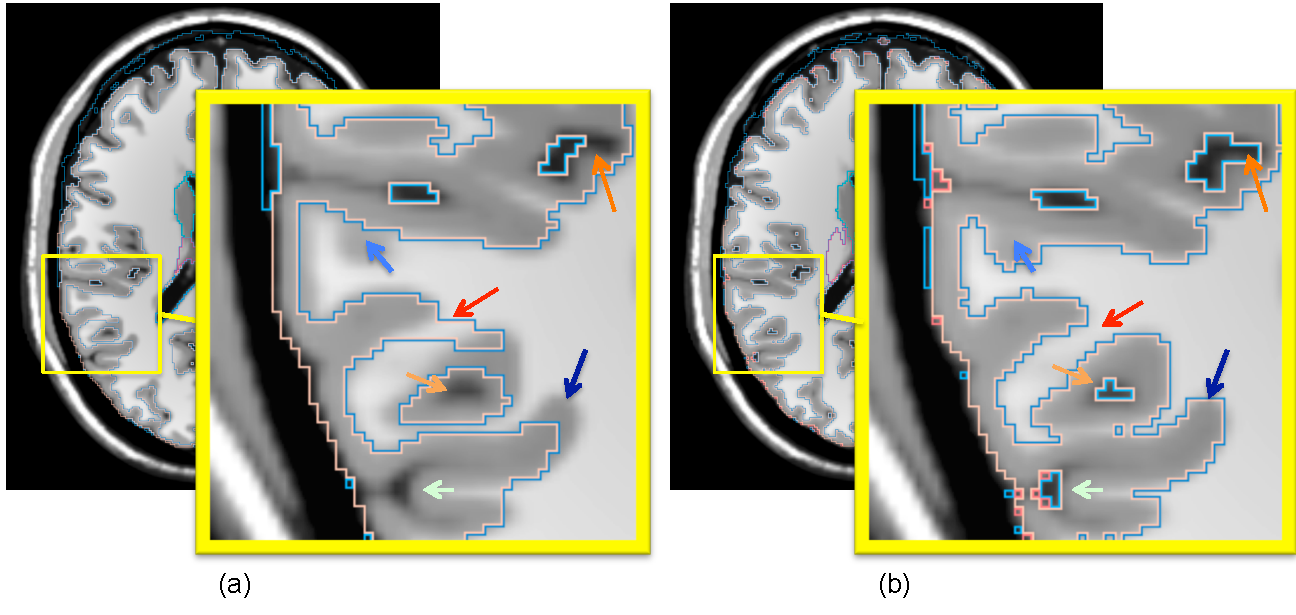
\includegraphics[width=6.75in,height=3.3in]{useKNN_qualitative}\
\centering
\caption{Visual comparison of segmentation results on a sample PREDICT-HD MR data between (a) $EM$ only based classification and (b) proposed enhancements using a fuzzy $k-NN$ classifier. More accurate delineation is achieved by the proposed approach.}
\label{useKNN_qualitative}
\end{figure}
%--------------------------------

%--------------------------------
\begin{figure}
\centering
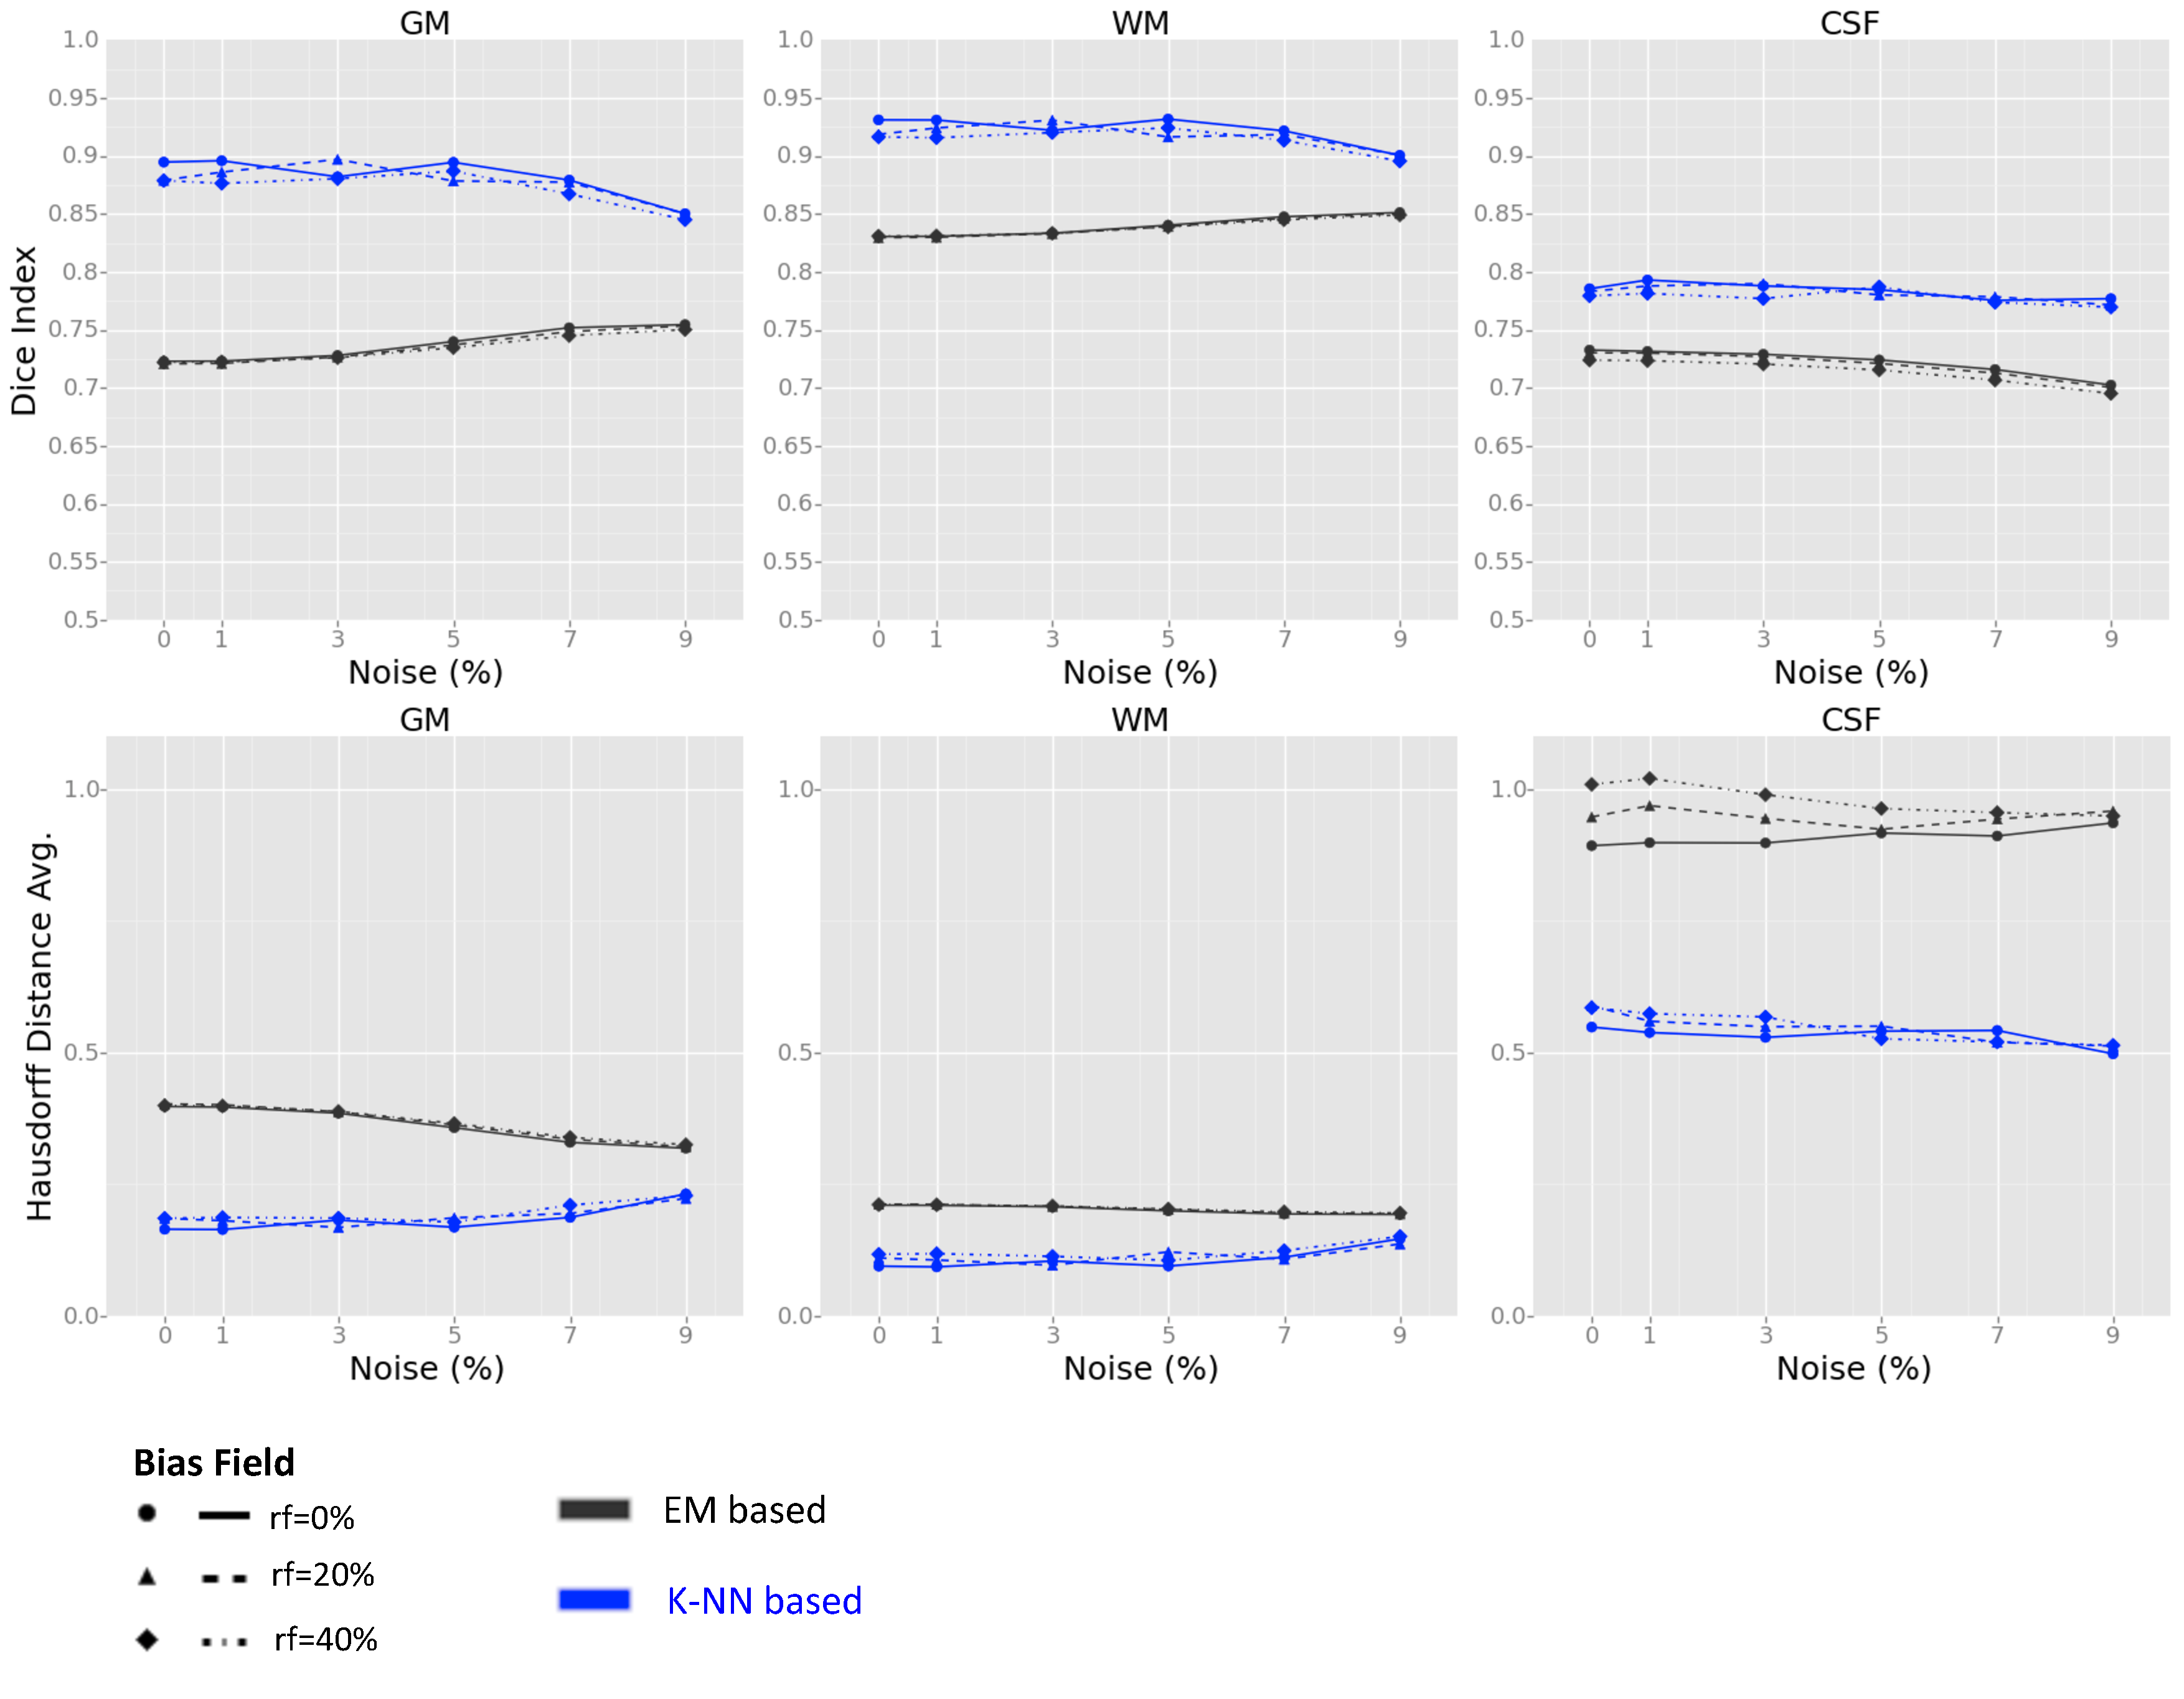
\includegraphics[width=6.75in,height=5.5in]{kNN_vs_EM}\
\centering
\caption{Comparison of the classification of cerebrospinal fluid (CSF), Grey matter (GM) and White matter (WM) tissues between $EM$ only based classification (black) and the extended method by a fuzzy $k-NN$ classifier (blue) using two independent measures, Dice index (larger is better) and average Hausdorff distance (smaller is better) . The evaluation is performed along three degrees of bias-field (rf=0, rf=20 and rf=40) and six levels of noise ($0\%$, $1\%$, $3\%$, $5\%$, $7\%$, and $9\%$) along x-axis. Both similarity measures show improvement on the results of the proposed $k-NN$ enhancements.}
\label{kNN_vs_EM}
\end{figure}
%--------------------------------

\paragraph{Discussion and Conclusions} %-----------------

This work improved automated classification of brain tissues for multi-center $3D$ MRI data analysis. Previous studies have used expectation maximization (EM) based classification that is group specific and uses a \emph{priori} knowledge for all the subjects in an atlas based approach.
This paper, however, emphasized the importance of a non-parametric model's utility in neurodegenerative diseases, since each subject has unique anatomical states in longitudinal degenerative studies that may not be represented by prior probability distributions. Enhancements were suggested by augmenting the $EM$-based classification using a fuzzy k-nearest neighbor (k-NN) classifier that builds up a model for each individual subject and complements the classification results that $EM$ produces.
A Fuzzy $k-NN$ method was selected, as this non-parametric classifier is subject specific; it is not biased by prior probability distributions, and it potentially can model more complex decision boundaries than a Gaussian distribution based mixture method.

The proposed implementation generates more precise results than $EM$ only classification, since both similarity measures, Dice index and the average Hausdorff distance, show improvement on the results of $k-NN$ classifier as demonstrated in Figure \ref{kNN_vs_EM}.
Also, qualitative observations in Figure \ref{useKNN_qualitative} show that our method especially provides more accuracy in delineation of sophisticated tissue boundaries where tissue regions are highly interleaved together like GM and WM boundaries.
\newline

\subsubsection{Research Design for Aim 1 Subtask 2: Enhance multi-modal classification when complementary information comes from a second modality with lower spatial resolution}
\label{section:Aim1Subtask2ResearchDesign} %--------------------

Previous subtask suggested enhancements when both $T1$/$T2$-weighted $MR$ modalities were acquired at the same high spatial resolution with isotropic $1$ $mm^{3}$ voxel sizes. However, many real world data are collected such that $T2$ image is acquired in lower spatial resolution than $T1$ (usually by a factor of $2$ to $3$). This is especially the case in datasets provided from scanners with $1.5$ Tesla scan protocol.

The enhanced multi-modal classification framework in section \ref{section:Aim1Subtask1ResearchDesign} operates in voxel lattice space. It would not cause any problem if always all input modality scans were provided at the same voxel space. However, now we need to enhance the previous infrastructure to run in physical space before we investigate the segmentation results in the case that input modality scans are not in the same resolution and their voxel lattices do not line up.

In this section, first we enhance the presented multi-modal classification framework to run in physical space, and we demonstrate that the system is upgraded successfully by generating equivalent results in single-modal mode. 
Then, we show that na\"{i}vely adding the information of a second modality with lower spatial resolution can worsen the segmentation results. We investigate and explain the reason by describing partial volume effects (PVE). Finally, we propose a novel approach to deal with PVE issue and evaluate the proposed method.

\paragraph{Enhance classification framework to run in physical space} %--------------------

In a multi-modal classification framework different modalities may have different resolutions.
Therefore, it is important to perform classification in physical space to avoid interpolation errors that may introduce artificial partial volume effects.
In this step, classification framework is reimplemented to perform in physical space.

\subparagraph{Evaluation}
Only T1 modality is used to evaluate the performance of the reimplemented framework. By using only one modality, we expect to get the same results as the classification was run in voxel space vs. physical space. 
Again BrainWeb dataset, as described in section \ref{brainWebData}, was used for quantitative evaluation of the classification performance.

\subparagraph{Results}
Figure \ref{Use_physical_space} reports the ``Dice Index'' measure to compare the results of the automated delineations against the ground truth when the algorithm was run in voxel space vs. physical space.

\subparagraph{Conclusion}
Single-modal results show that there is no difference in the performance when the algorithm was run in physical space rather than voxel space, which is good since it means we did not spoil the results when the framework was upgraded. Now we are ready to do further investigations using the prepared classification infrastructure.

%--------------------------------
\begin{figure}[ht]
\centering
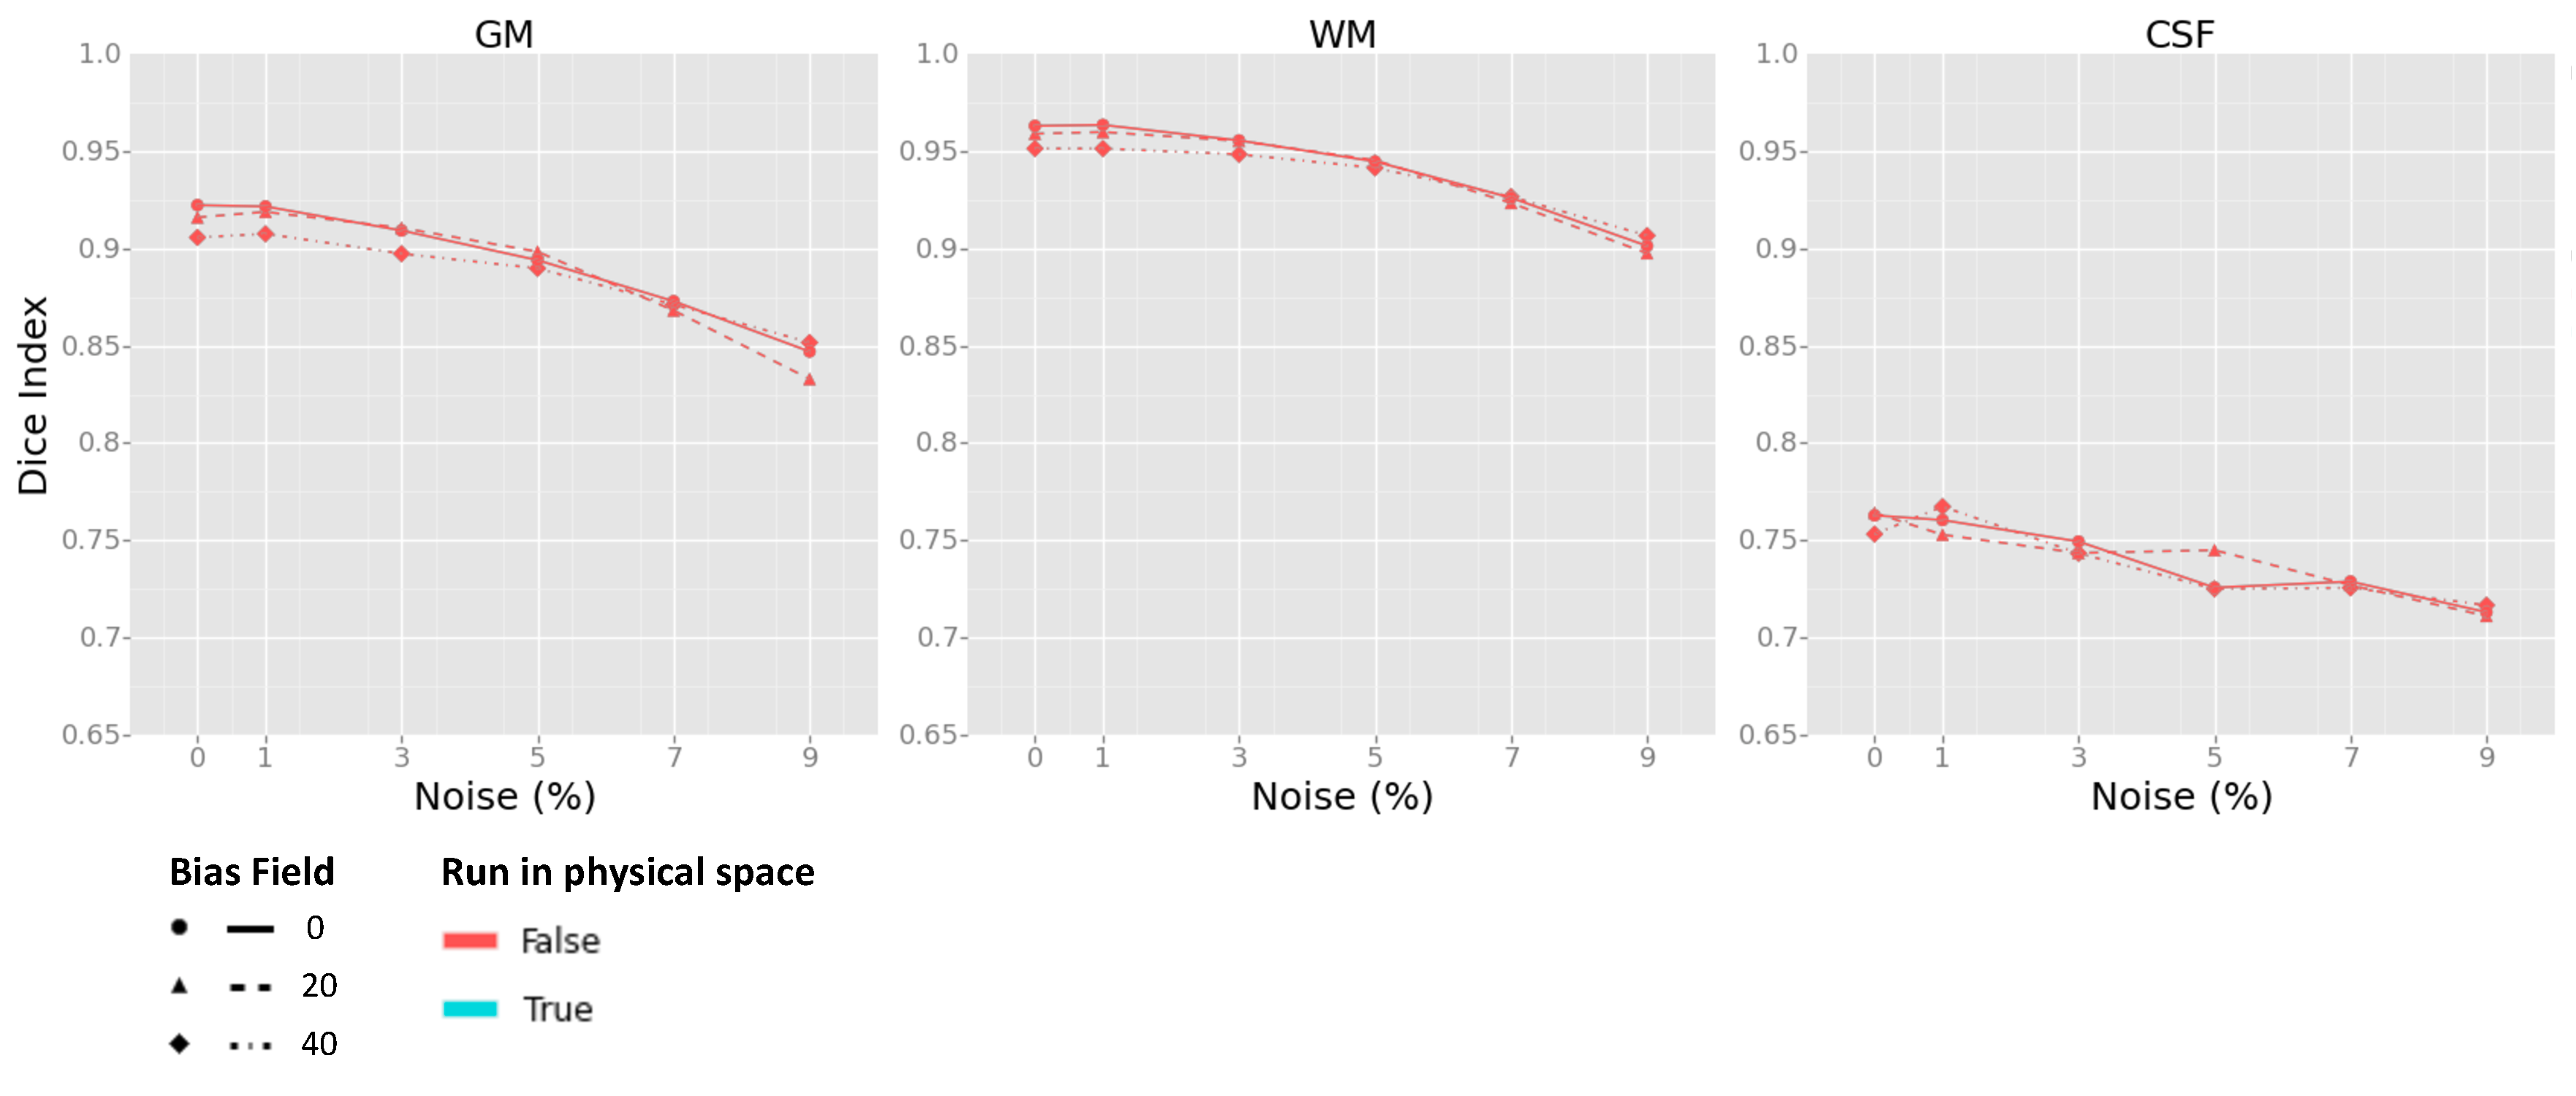
\includegraphics[width=7.6in,height=3.3in]{Use_physical_space}\
\centering
\caption{The classification framework generates essentially the same results in single-modal mode when it is run in physical space versus voxel space, since blue and red lines are almost overlapped.} 
\label{Use_physical_space}
\end{figure}
%--------------------------------

\paragraph{Significance}

It is well established that multi-modal MR images can provide complementary information that can improve brain tissue classification \cite{Kim2013}. 
However, this does not hold when the additional information comes from a second modality provided in low spatial resolution.

It is demonstrated in Figure (\ref{T2_1x1x1_vs_T2_1x1x3}) by running two multi-modal experiments using two $T1$ and $T2$ MR modalities. \textit{Green} color shows the results when both modalities have the same isotropic $1$ $mm^3$ resolution, while the results from two modalities with different resolutions are shown in \textit{blue} color, where $T1$ is provided with isotropic $1$ $mm^3$ resolution, but T2 has $1 \times 1 \times 3$ $mm^3$ voxel sizes.

%--------------------------------
\begin{figure}
\centering
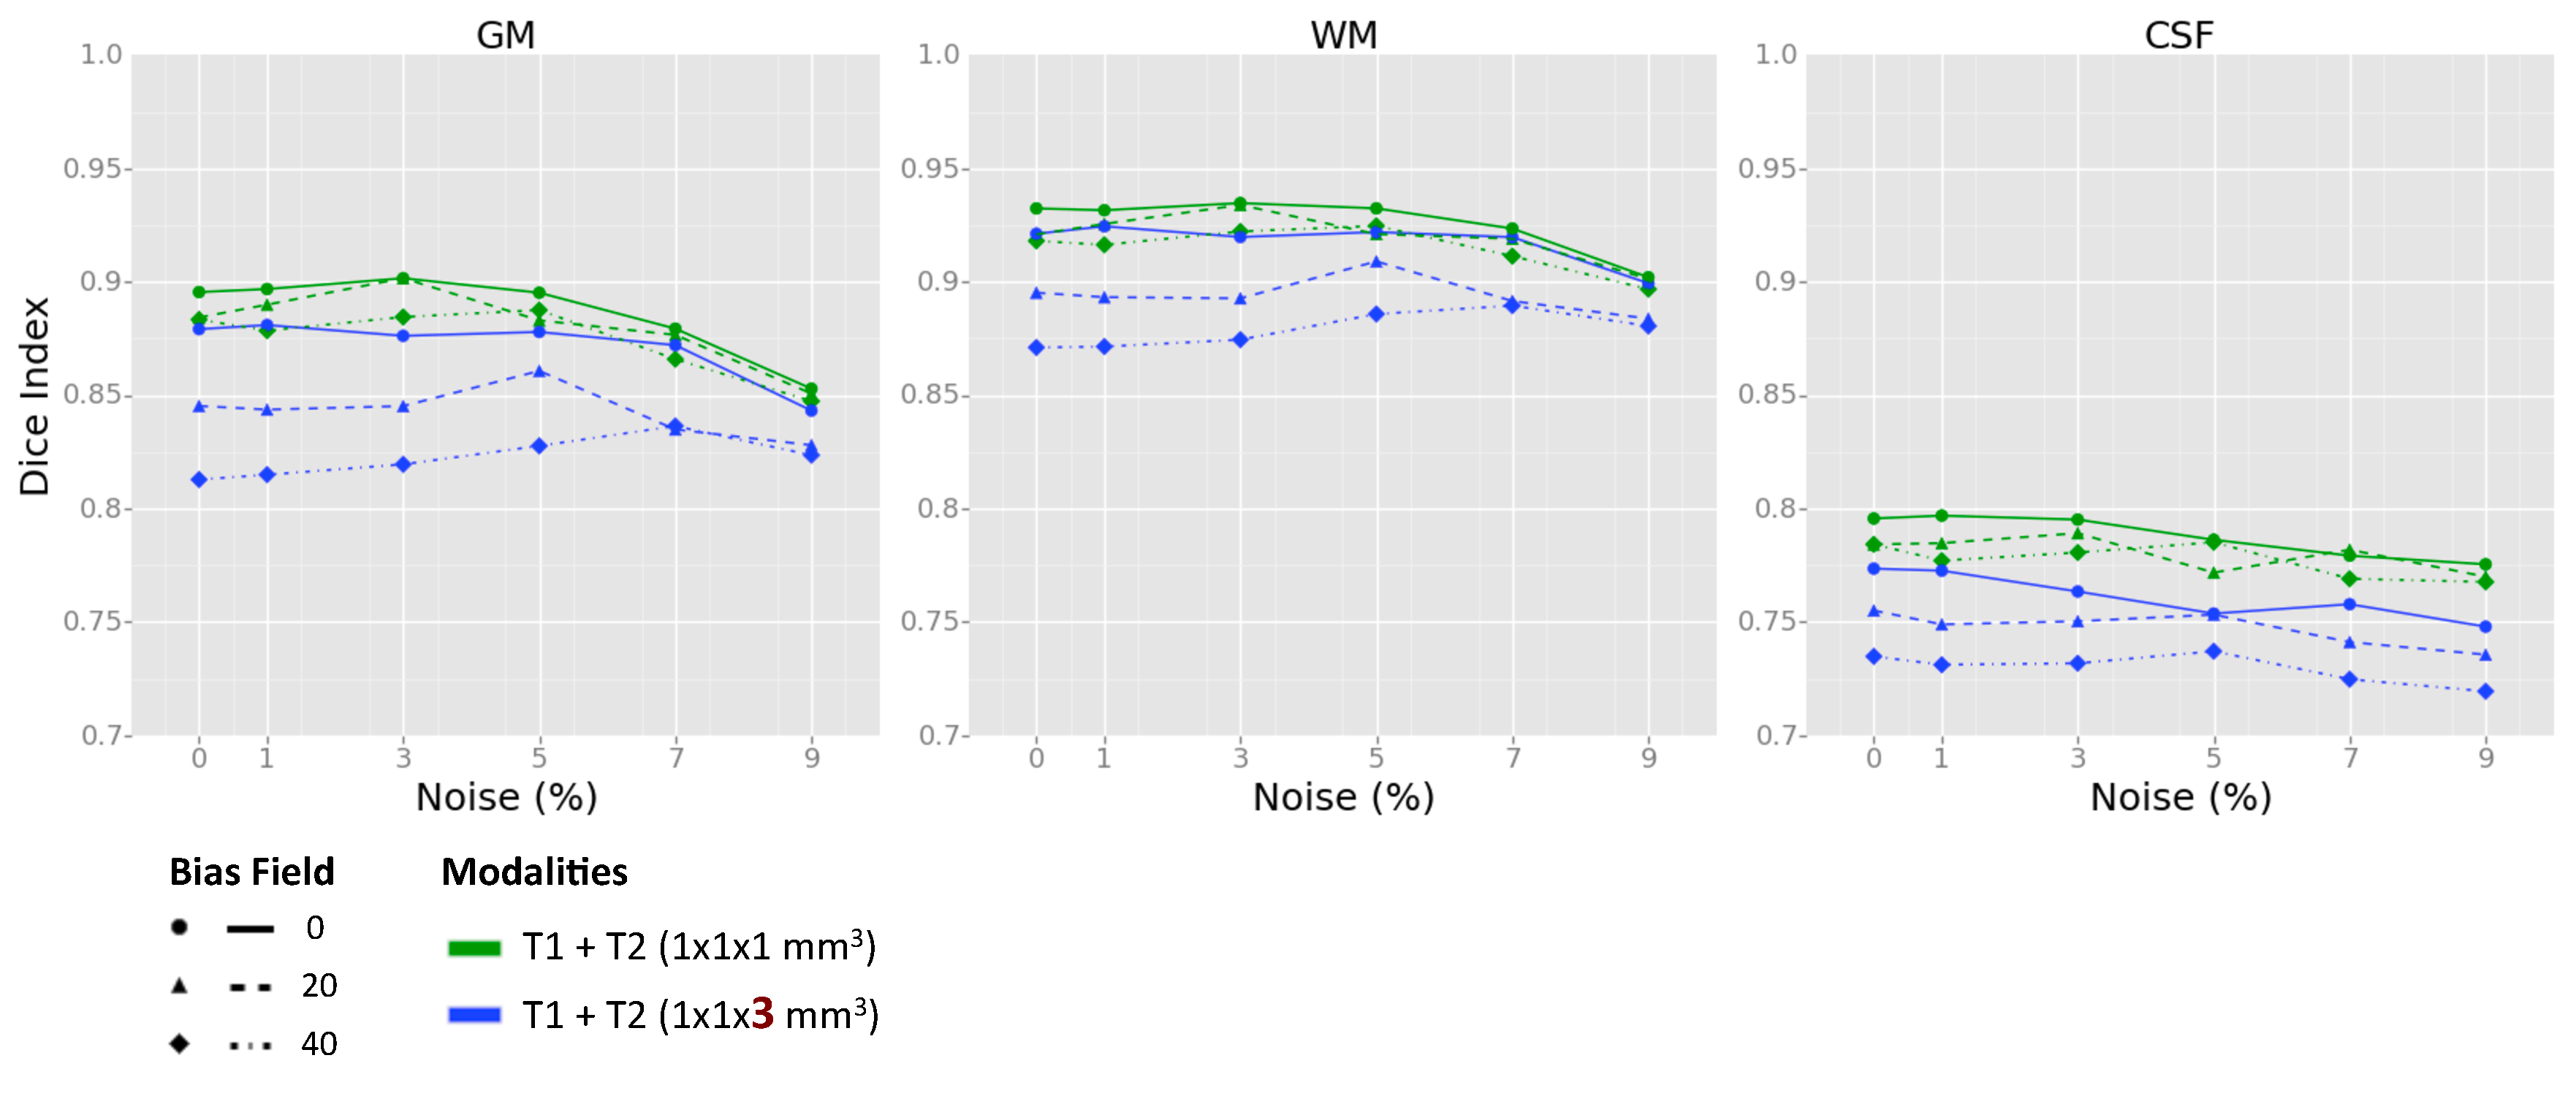
\includegraphics[width=7.6in,height=3.3in]{T2_1x1x1_vs_T2_1x1x3}\
\centering
\caption{Blue lines show worse classification results when second modality ($T2$: $1 \times 1 \times 3$ $mm^3$) has lower resolution than the first modality ($T1$: $1 \times 1 \times 1$ $mm^3$).} 
\label{T2_1x1x1_vs_T2_1x1x3}
\end{figure}
%--------------------------------

Figure (\ref{T2_1x1x1_vs_T2_1x1x3}) shows that adding information from a second modality with significantly lower resolution decreases the quality of the segmentation results.
It is expected because misalignment between voxel sizes and voxel locations increases \textit{partial volume effect} (PVE) at tissue boundaries that means more spatial samples at the boundaries contain a mixture of tissue types. Using these voxels to initialize $EM$ parameters and to train $KNN$ algorithm can adversely affect the performance of the classifier and results in less accurate and less robust tissue classification.

\subparagraph{Partial Volume Effect}

Due to the finite spatial resolution of the imaging device, a single image voxel may contain of several tissue types. This phenomenon, termed as partial volume effect (PVE), complicates the segmentation process, and, due to the complexity of human brain anatomy, dealing with the PVE issue is an important factor for accurate brain structure classification.

Figure (\ref{fig:pve}) shows a schematic explanation of the partial volume effect in a simplified $1D$ demonstration, where $1D$ MRI signals from three different image modalities (T1, T2 and DWI) are demonstrated near actual anatomical boundaries of Gray matter and White matter in brain.
The MRI works by detecting the magnetic particles in atoms within cells and sending electromagnetic pulses at different rates and strength through the body. Then different types of matter give off different levels of energy when they are placed in a magnetic field. These energy signals, collected by the electromagnetic receivers, are quantized and sampled into discrete voxel segments in an output image scan. The different signal levels between different tissue types cause each matter shows a different contrast in the output image. In an MRI scanning session, a number of different scans are run. Depending on how they measure the relaxation of the magnetic particles, a variety of modality images with different contrasts are acquired. For example, in a T1 scan, gray matter gives off a low signal and looks darker than the white matter that gives off a higher signal and looks pale gray, but this is inverse in T2 and DWI scans.

Although objects of interest usually form coherent continues shapes with clear anatomical borders, the representation of tissue boundaries in discretized image scan is not perfectly in agreement with real anatomy because of error in image discretization. In fact, biology cannot conform in the resolution levels that scanners produce.

First, the measurement of MRI signals is not perfect due to the hardware limitations and the presence of noise in the input image, so the collected signals are quantized in several intermediate levels in boundary regions. This causes an inherent partial volume effect at tissue boundaries even in a single modality acquisition.
The quantized signals are then mapped in discretized segments of spatial domain. A value is assigned to each voxel of the image based on the average of samples taken within the spatial range of that voxel. 
If the image has a low spatial resolution with large voxel sizes, it is most likely that many voxels are placed in two different anatomical regions, so their value reflects a partial volume composition of more than one tissue type.

Partial volume composition affects a larger number of spatial samples when the multi-modal information comes from the modality scans having different resolutions and origins.
In Figure (\ref{fig:pve}), the MRI signals are sampled in $1$ $mm$ intervals. 
When only two T1 and T2 modalities with comparable resolutions are used, we have more pure spatial samples since only two samples are affected by partial volume composition (specified in a red box). 
However, adding new modality information from a low resolution scan introduces the partial volume effect to a larger number of spatial samples. The affected samples are specified in a green box and represented by a question mark as they reflect more than one tissue type.

A careful consideration should be made to only use those spatial samples that are not affected by partial volume composition, termed as \textit{pure samples}, for the initializing/training of the classification modules.

%--------------------------------
\begin{figure}
\centering
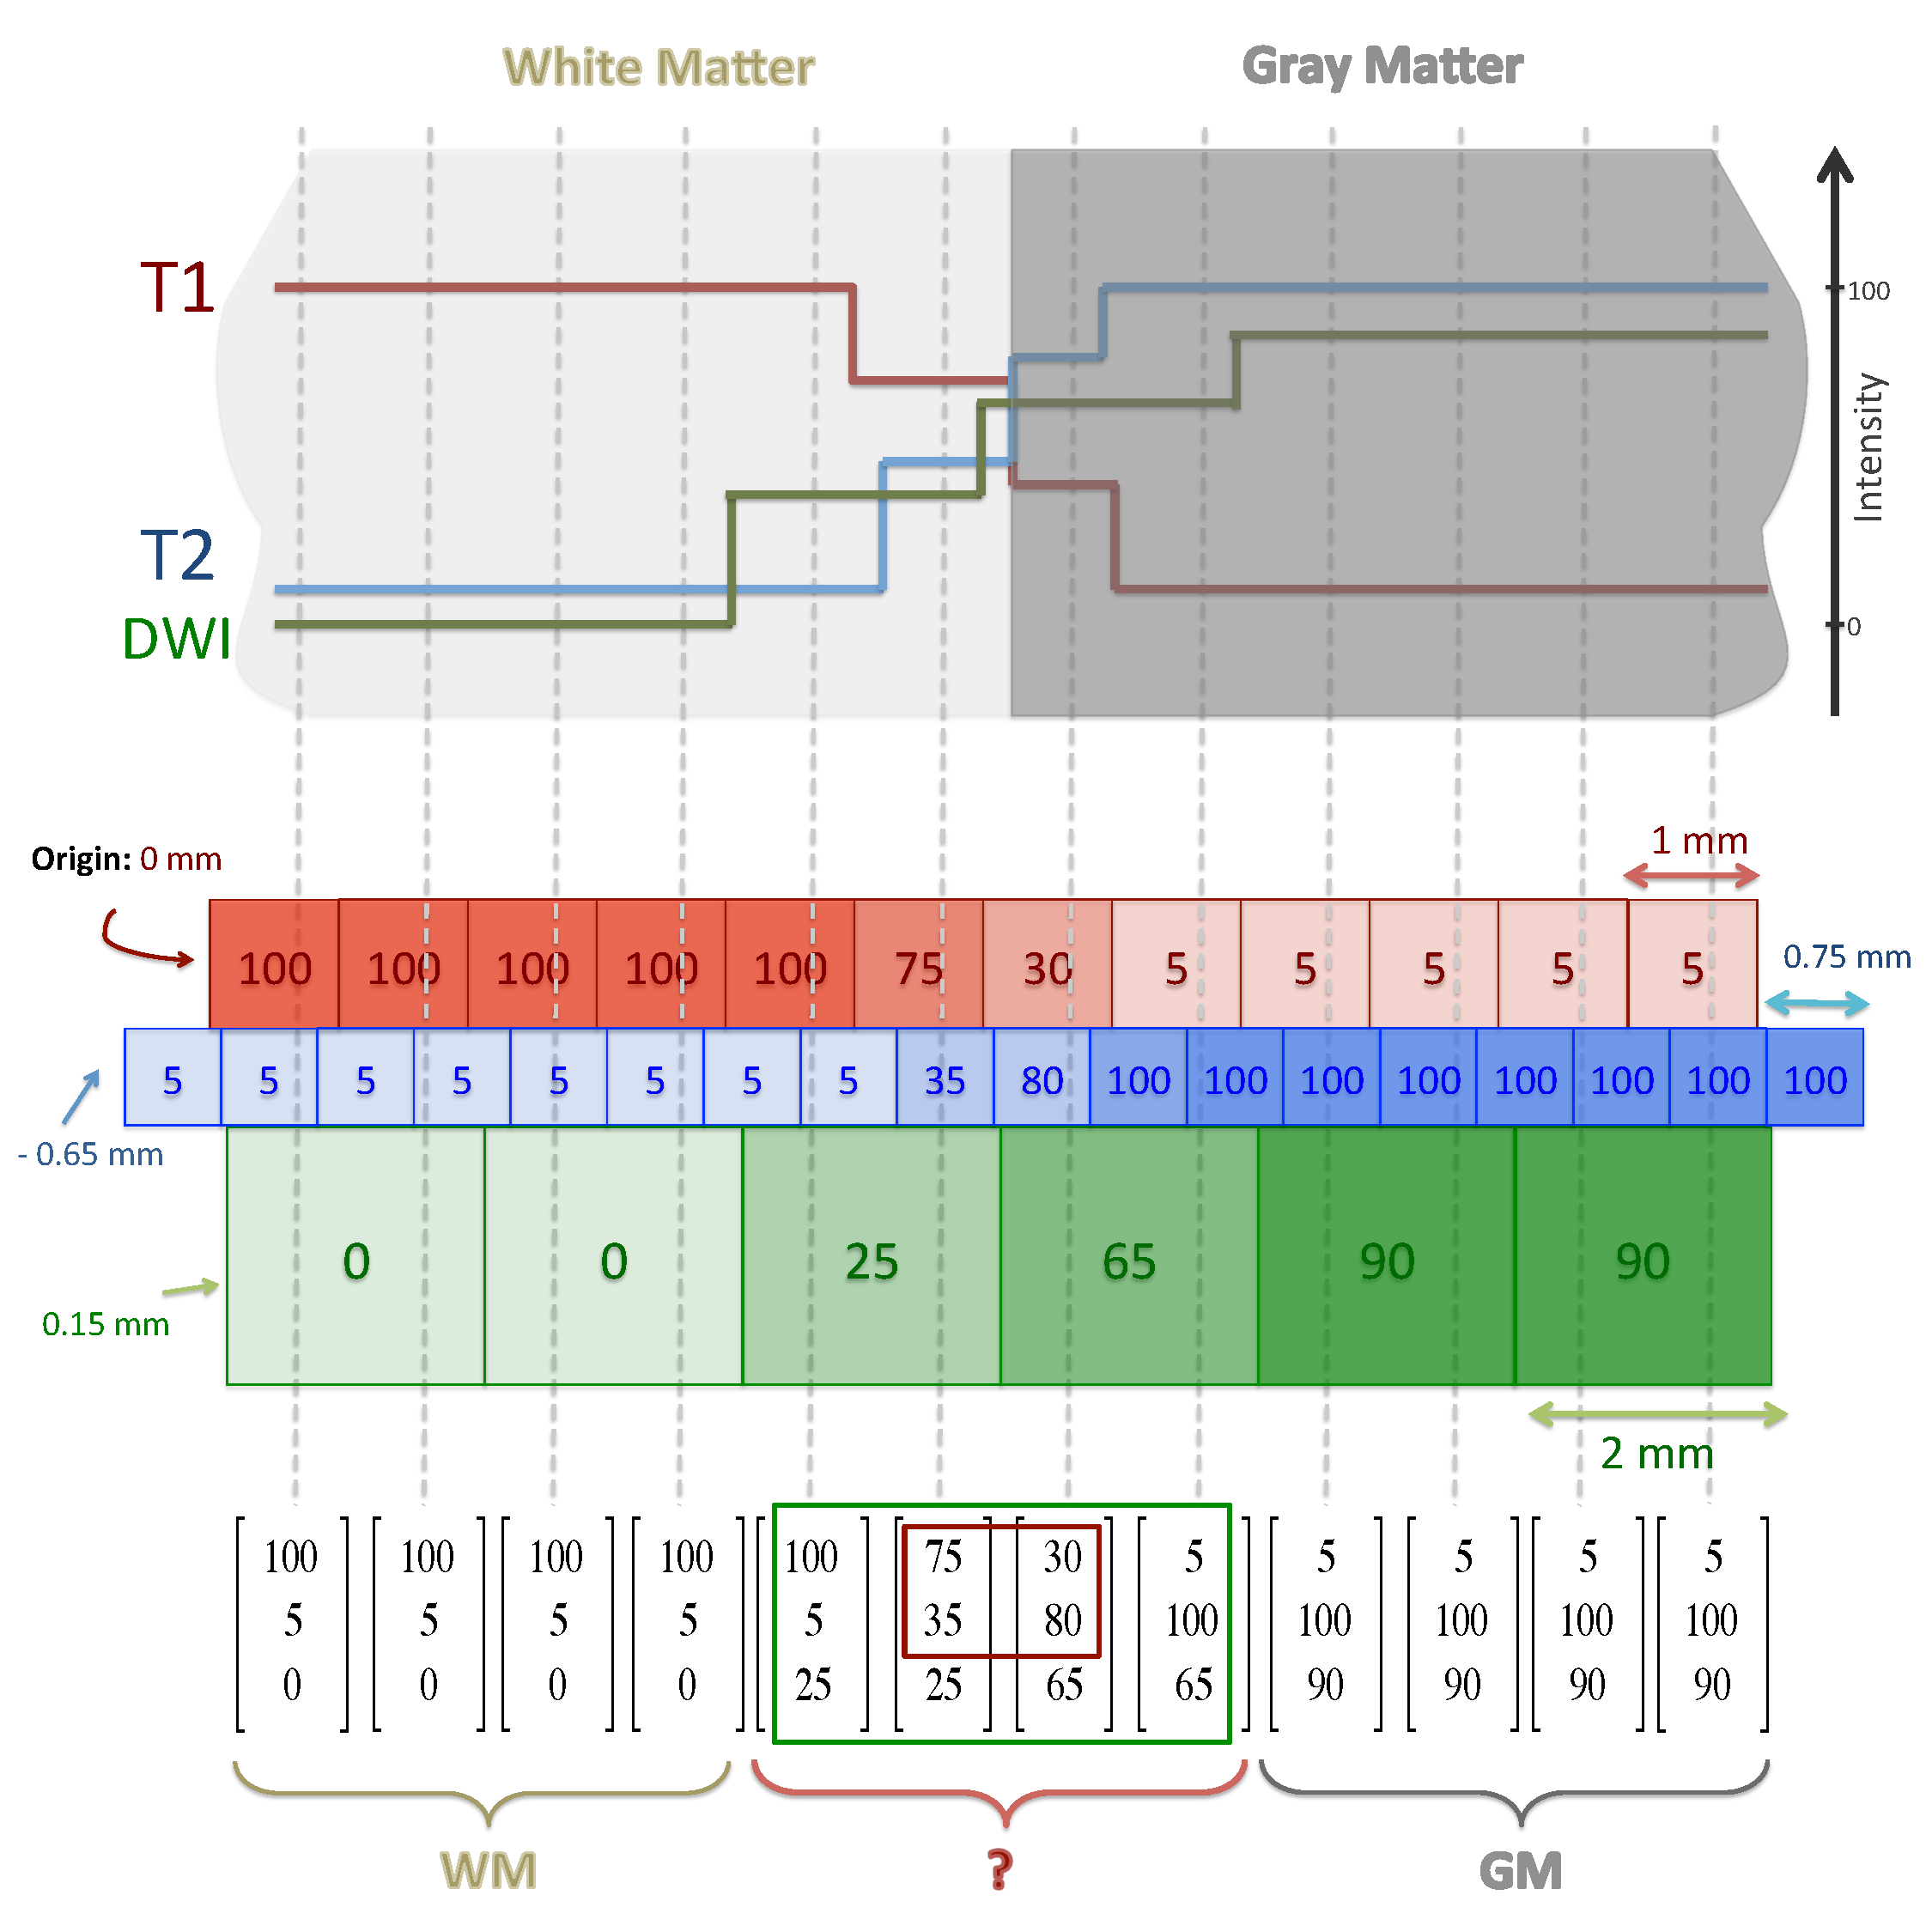
\includegraphics[width=5.6in,height=5.4in]{pve}\
\centering
\caption{$1D$ demonstration of partial volume effect (PVE) when MRI signals of different modalities are sampled to discredited segments with different spatial resolution and origin. Question mark represent the sample values that reflect a partial volume composition of more than one tissue type.} 
\label{fig:pve}
\end{figure}
%--------------------------------

\paragraph{Approach} %--------------------------------

Classification accuracy can be improved by excluding the voxels affected by the partial volume composition, termed as \textit{mixed samples}, from the initialization of the $EM$ algorithm and the training of the $KNN$ classifier.
Figure (\ref{fig:scatter_map}) demonstrates the scatter maps of the pure samples versus the mixed samples in a coronal view of two Gray matter and White matter tissue regions.

%--------------------------------
\begin{figure}
\centering
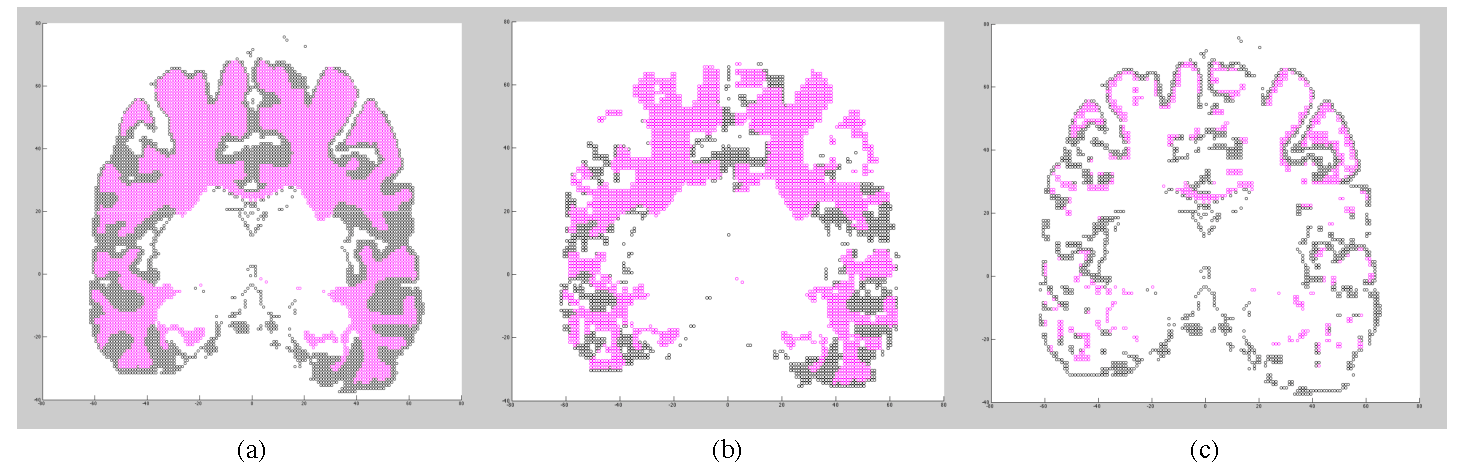
\includegraphics[width=6.36in,height=2.06in]{scatter_map}\
\centering
\caption{(a) a coronal view of a scatter point map of two Gray matter (black) and White matter (pink) tissues. (b) pure samples only. (c) mixed samples only.} 
\label{fig:scatter_map}
\end{figure}
%--------------------------------

In this section, we propose a new approach to identify the pure samples by computing a binary mask, called \textit{pure plugs mask}, that excludes all the mixed samples from the initialization/training of the classification methods.

\subparagraph{Computing pure plugs mask}

To compute a pure plugs mask, we should avoid both inherent PVE at tissue boundaries and the PVE caused by information inconsistency through multiple modality channels.
%Following steps are proposed to compute a pure plugs mask:

\subparagraph*{1) Avoid inherent PVE}
All the voxels located in tissue boundaries may include a mixture of both tissue regions since the biology cannot conform in the resolution levels that scanners produce. This inherent partial volume effect is avoided by excluding all tissue boundaries from the pure plugs mask. For this purpose, anatomical edges are detected from the input modality with the finest resolution (usually a $T1$-weighted scan) using a Canny edge detector \cite{canny1986} as shown by Figure (\ref{fig:canny_edge_mask}).

%--------------------------------
\begin{figure}
\centering
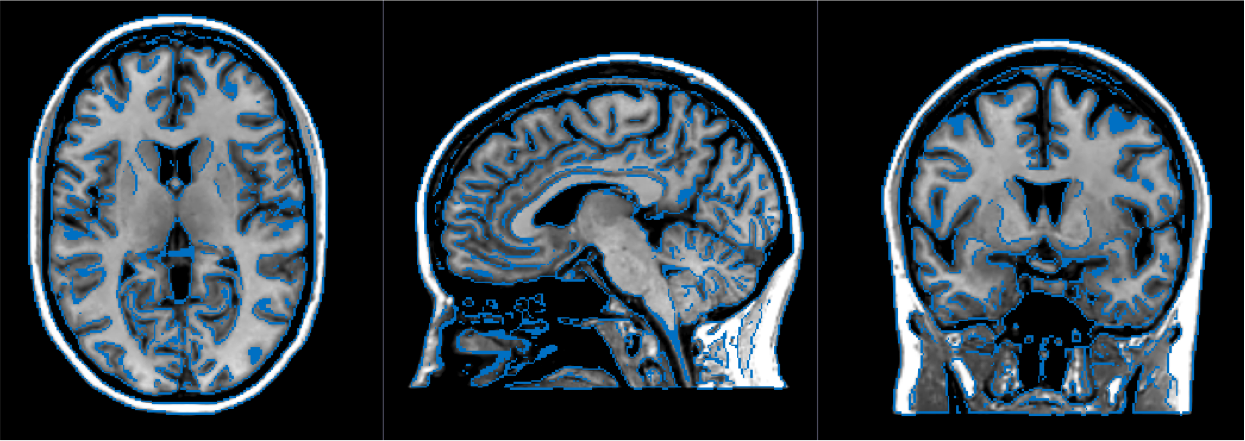
\includegraphics[width=5.5in,height=2in]{canny_edge_mask}\
\centering
\caption{Anatomical tissue boundaries are detected using a Canny edge detector. Detected edges should be excluded from the pure plugs mask to avoid inherent PVE in tissue boundaries.} 
\label{fig:canny_edge_mask}
\end{figure}
%--------------------------------

\subparagraph*{2) Avoid multi-modal PVE}
As demonstrated by Figure (\ref{fig:pve}), partial  volume  composition  affects  a  larger  number  of  spatial  samples  when  the  multi-modal  information comes from multiple modality scans with different voxel resolutions. 
To deal with this issue, only pure samples should be included in the classification process. To find the pure samples, \textit{pure plugs} should be computed.

\subparagraph*{What is a pure plug?}
A \textit{pure plug} is defined as a region (plug), where all multi-modal images have consistent information within the entire range of that region. The size of each plug region is then decided based on the lowest spatial resolution at each direction within all the input modality scans.

This definition raises an immediate question: how do we define the consistency of multi-modal information within a plug region? This is discussed in following section by defining the \textit{pure plugs integrity metric}.

However, before analysing the information from multi-modal channels, all the input images should to be normalized to have the same dynamic range for their intensity values.

\subparagraph*{Standardize intensity}

An intensity transformation function, as shown in Figure (\ref{fig:standardizeIntensity}), is applied to the intensity levels of each input image. All the input modality scans are scaled to have the same dynamic range based on the first and last $5$ percentiles of their histogram. Also, low and high tails of data in the output image are trimmed to the constant bounds of $0$ and $1$. This transform function can formulated as:

\begin{equation}
\label{eq:standardizeIntensity}
\begin{gathered}
O(i) = \begin{cases}
\alpha I(i) + b_{0} & \text{ if   } \frac{-b_0}{\alpha} < I(i) < \frac{1-b_0}{\alpha} \\ 
1 & \text{ if } I(i) > \frac{1-b_0}{\alpha} \\ 
0  & \text{ if } I(i) < \frac{-b_0}{\alpha} 
\end{cases} \\
\quad where \quad \alpha = \frac{0.9}{ Q_I(95) - Q_I(5) } 
\text{  ,  } b_0 = 0.95 - Q_I(95) . \alpha
\end{gathered}
\end{equation}

Where at index $i$, $O(i)$ is the output image intensity, $I(i)$ is the input image intensity, and $Q_I(p)$ is the $p^{th}$ quantile (percentile) of the input intensity range.

%--------------------------------
\begin{figure}
\centering
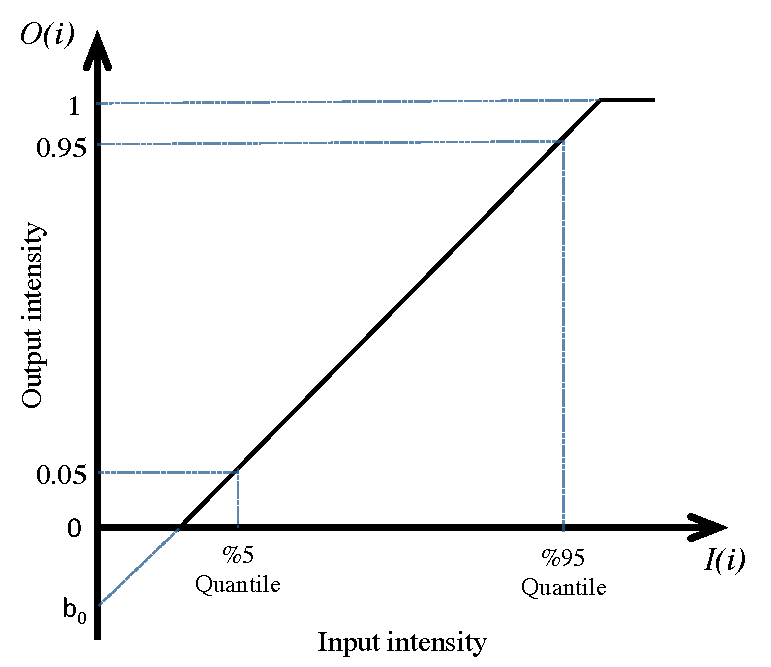
\includegraphics[width=3.45in,height=3in]{standardizeIntensity}\
\centering
\caption{Intensity transform function applied to each input modality image to make all the input images have the same intensity dynamic range.} 
\label{fig:standardizeIntensity}
\end{figure}
%--------------------------------

\subparagraph{Pure plugs integrity metric}

To decide whether a plug is considered pure or not, we will pick several spatial sample points uniformly distributed within the entire range of the plug area. Then, each sample point is represented in an $N$-dimensional intensity space based on the normalized intensity values from $N$ input modality channels.

Figure (\ref{fig:four_tissues_jh_points}) shows a joint image histogram for two input modality, $T1$ and $T2$, images.
The picture shows the distribution of points in different colors for background and four tissue regions (White Matter (WM), Gray Matter (GM), Cerebrospinal Fluid (CSF), and Venous Blood (VB)).
It is critical to notice that for a single tissue region, the points are distributed non-uniformly in different directions. The reason is that the input modality scans have different variance for the intensity ranges within a tissue region.

%--------------------------------
\begin{figure}
\centering
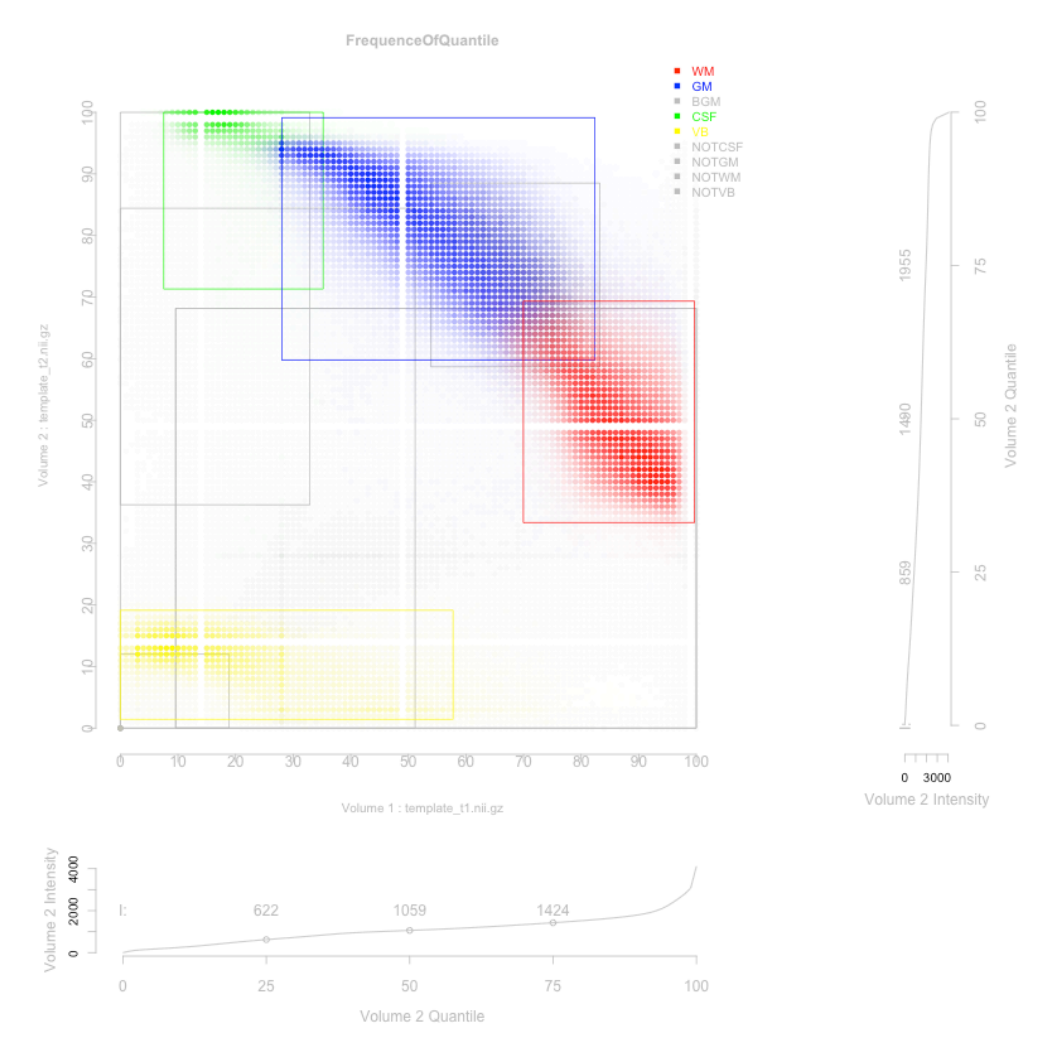
\includegraphics[width=6in,height=6in]{four_tissues_jh_points}\
\centering
\caption{Joint image histogram for two modality images. The distribution of points is shown in different colors for background (grey) and four tissue regions: White Matter (red), Gray Matter (blue), Cerebrospinal Fluid (green), and Venous Blood (yellow). A box is plotted around the mean of each region with the size of 4 standard deviation at each direction.} 
\label{fig:four_tissues_jh_points}
\end{figure}
%--------------------------------

Therefore, the spatial sample points, that are picked within a plug region, may not be uniformly distributed in the intensity space even if all belong to a single tissue region.
Hence, a metric should be defined to decide about the integrity of the sample points based on following criteria:

\begin{itemize}
    \item[-] Detects the possible outliers in the sampled points distribution.
    \item[-] Considers the sparsity of the sampled points. 
\end{itemize}

The shape and size of the multivariate sample points can be quantified by the covariance matrix. A well-known distance measure that takes into account the covariance matrix is the \textit{Mahalanobis distance}, so it is used as the basis for multivariate outlier detection \cite{filzmoser2004}. 
For an $N$-dimensional sample $\bar{X}_k = (x_1, x_2, ..., x_N)^{T}$ in a set of observations, the Mahalanobis distance is defined as:

%--------------------------------
\begin{equation}
\begin{gathered}
D_M(\bar{X}_k)=\sqrt{(\bar{X}_k-\bar{\mu})^T S^{-1} (\bar{X}_k-\bar{\mu})}
\end{gathered}
\end{equation}
%--------------------------------

Where $S$ is the covariance matrix, and $\bar{\mu} = (\mu_1, \mu_2, ..., \mu_N)^{T}$ is the mean of all observations.
Essentially the Mahalanobis distance is an Euclidean distance that considers the covariance of the data by down-weighting the axis with higher covariance.

Then, a sample $\bar{X}_n$ is considered as outlier, if $D_M(\bar{X}_n) > \alpha.Mean(D_M)$, where $\alpha$ can tune the threshold value.

Although the Mahalanobis distance is useful to detect the outliers, it is not a good integrity metric for finding the pure plugs, as it is scale invariant. This means that Mahalanobis distance does not consider how sparsely the sample points are distributed. Figure (\ref{fig:md_scale_invar}) shows this in an example.

%--------------------------------
\begin{figure}
\centering
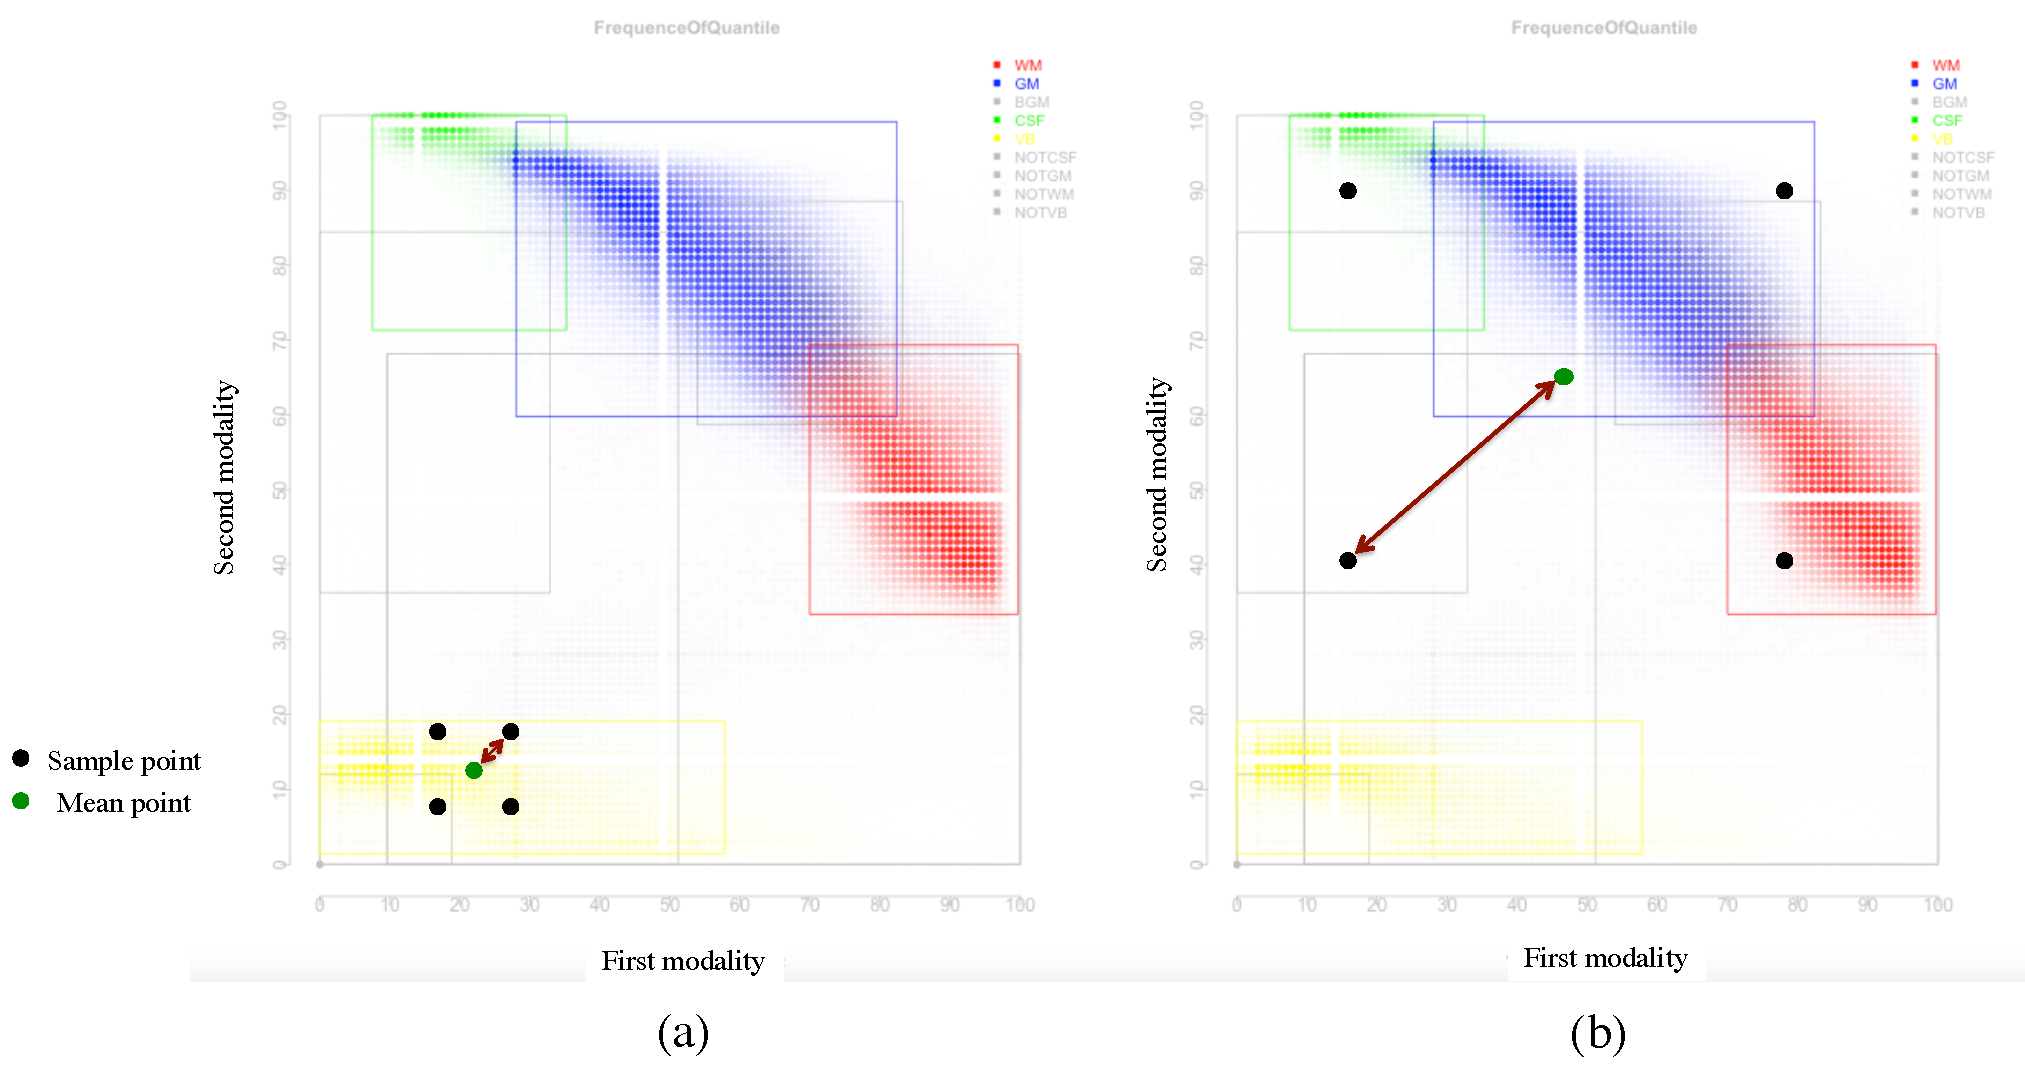
\includegraphics[width=6.75in,height=3.6in]{md_scale_invar}\
\centering
\caption{Mahalanobis distance is scale invariant and does not consider the sparsity of points. (a) The Mahalanobis distance for all points is $1.22$, and all points belong to a single tissue region. (b) Again the Mahalanobis distance for all points is $1.22$, but points belong to four different regions.} 
\label{fig:md_scale_invar}
\end{figure}
%--------------------------------

To consider the sparsity of the points, an \textit{Euclidean distance} can be used to show how dense all the sample points are scattered within an intensity range of $0<i<1$. Therefore, the integrity metric can be defined as the combination of both \textit{Mahalanobis} and \textit{Euclidean} distance measures, such that:

\begin{itemize}
    \item[-] Mahalanobis distance can find outliers considering the covariance of distribution.
    \item[-] Euclidean distance can detect density of points within a threshold value.
\end{itemize}

In the proposed metric, the normalized Mahalanobis distance can be used to weight the Euclidean distance for each point. The integrity metric, called \textbf{Mahalanobis-weighted Euclidean distance}, is defined as:

%--------------------------------
\begin{equation}
\label{eq:integrityMetric}
\begin{gathered}
Dist(i) = \frac{M_D(i)}{Max(M_D)} \times E_D(i)
\end{gathered}
\end{equation}
%--------------------------------

Where, for the $i^{th}$ sample, $Dist(i)$ is the proposed integrity distance metric, $M_D(i)$ is the Mahalanobis distance, $E_D(i)$ is the Euclidean distance, and $Max(M_D)$ is the maximum Mahalanobis distance between all observations.

The computed integrity metric distance for all the sample points in Figure (\ref{fig:md_scale_invar} a) is $0.07$, which is significantly different compare to the distance metric of the sample points in Figure (\ref{fig:md_scale_invar} b) computed as $0.42$.

Based on the proposed distance metric in equation (\ref{eq:integrityMetric}), following steps should be taken at each plug region to decide whether it is pure or not:

\begin{itemize}
    \item[1)] Several spatial sample points are picked within each plug area, such that they are uniformly scattered over the entire region.
    \item[2)] All samples are transformed to an $N$-dimensional space based on their intensity values from $N$ input modality channels.
    \item[3)] The integrity distance measure, as in equation (\ref{eq:integrityMetric}), is computed for each sample point.
    \item[4)] The plug is then considered to be pure, if all the integrity distance values are less than a threshold that is defined as a value in the normalized intensity range (between $0$ and $1$).
\end{itemize}

The threshold value can be tuned based on the dataset. Here, we empirically chose a value of $0.2$. Figure (\ref{fig:pure_plugs_mask}) shows a test pure plugs mask created based on $3$ modalities from the dataset listed Table (\ref{PurePlugsMaskTestData}). This dataset was used as part of the multi-site international PREDICT-HD project. The third modality is an isotropic diffusion-weighted information ($IDWI$) image, that is geometric mean of diffusion images in the input $DWI$ dataset. This image has voxel sizes $8$ times bigger than conventional structural MR scans.

%--------------------------------
\begin{table}[ht]
\centering
\caption{Test dataset to create a test pure plugs mask}
\label{PurePlugsMaskTestData}
\begin{tabular}{|l|l|l|l|l|}
\hline
Scan        & Site                                                            & \begin{tabular}[c]{@{}l@{}}MR \\ vendor\end{tabular} & \begin{tabular}[c]{@{}l@{}}Field \\ strength\end{tabular} & \begin{tabular}[c]{@{}l@{}}Collected \\ modalities\end{tabular}                          \\
\hline \hline
0140\_52100 & 
\begin{tabular}[c]{@{}l@{}}Site\_024\\ (University of Iowa)\end{tabular} & 
SIEMENS TrioTim & 
3.0            & 
\begin{tabular}
[c]{@{}l@{}}T1: $1 \times 1 \times 1$ $mm^3$\\ T2: $1 \times 1 \times 1$ $mm^3$\\ IDWI: $2 \times 2 \times 2$ $mm^3$\end{tabular} \\ 
\hline
\end{tabular}
\end{table}
%--------------------------------

%--------------------------------
\begin{figure}
\centering
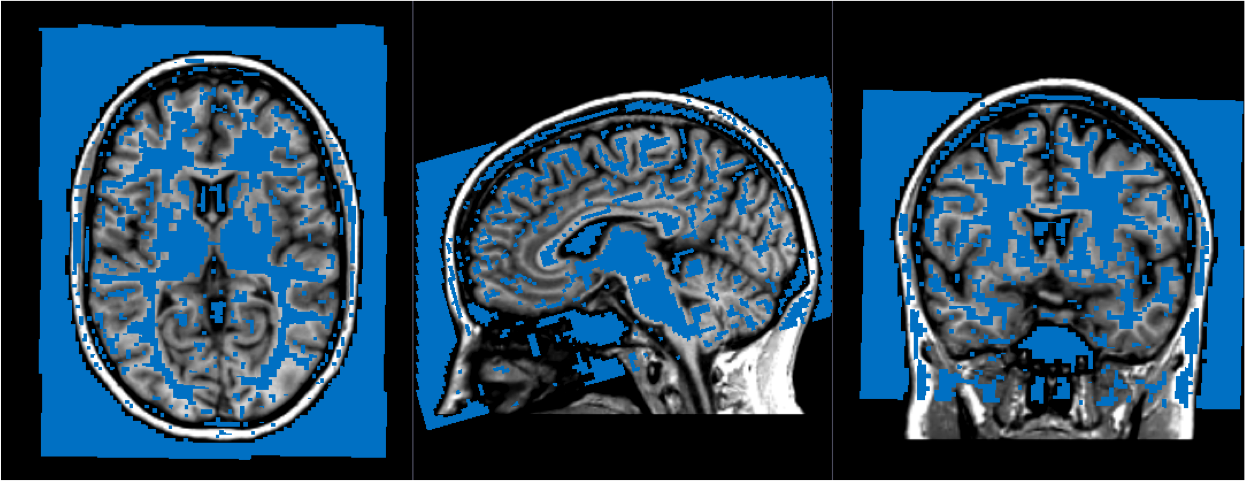
\includegraphics[width=5.5in,height=2in]{pure_plugs_mask}\
\centering
\caption{A test pure plugs mask created from $3$ modality scans from a subject test listed in table (\ref{PurePlugsMaskTestData}).} 
\label{fig:pure_plugs_mask}
\end{figure}
%--------------------------------

\paragraph{Experiments and Results}

Finally, we investigate how incorporating pure plugs mask can improve the segmentation results especially when input modalities are in different resolutions.

\subparagraph{Qualitative Evaluation} %-----------------

3D Slicer \cite{slicer_paper} was used to visually compare the previous segmentation results to the results of the proposed approach when only pure samples are used to initialize/train the classification methods.
Qualitative investigation was done using a sample dataset that was selected from a GE Signa $1.5$ Tesla scan protocol, where $T1$ resolution is $1 \times 1 \times 1$ $mm^3$, but $T2$ has the voxel sizes as $1.015 \times 1.015 \times 3$ $mm^3$.
This protocol was used as part of the multi-site international PREDICT-HD \cite{PREDICTHD} project.

Figure (\ref{fig:UsePurePlugs_qualitative}) shows the qualitative results. It shows that incorporating pure samples in the classification process can help detecting subtle tissue regions that were missed when the second modality has a lower resolution.

%--------------------------------
\begin{figure}
\centering
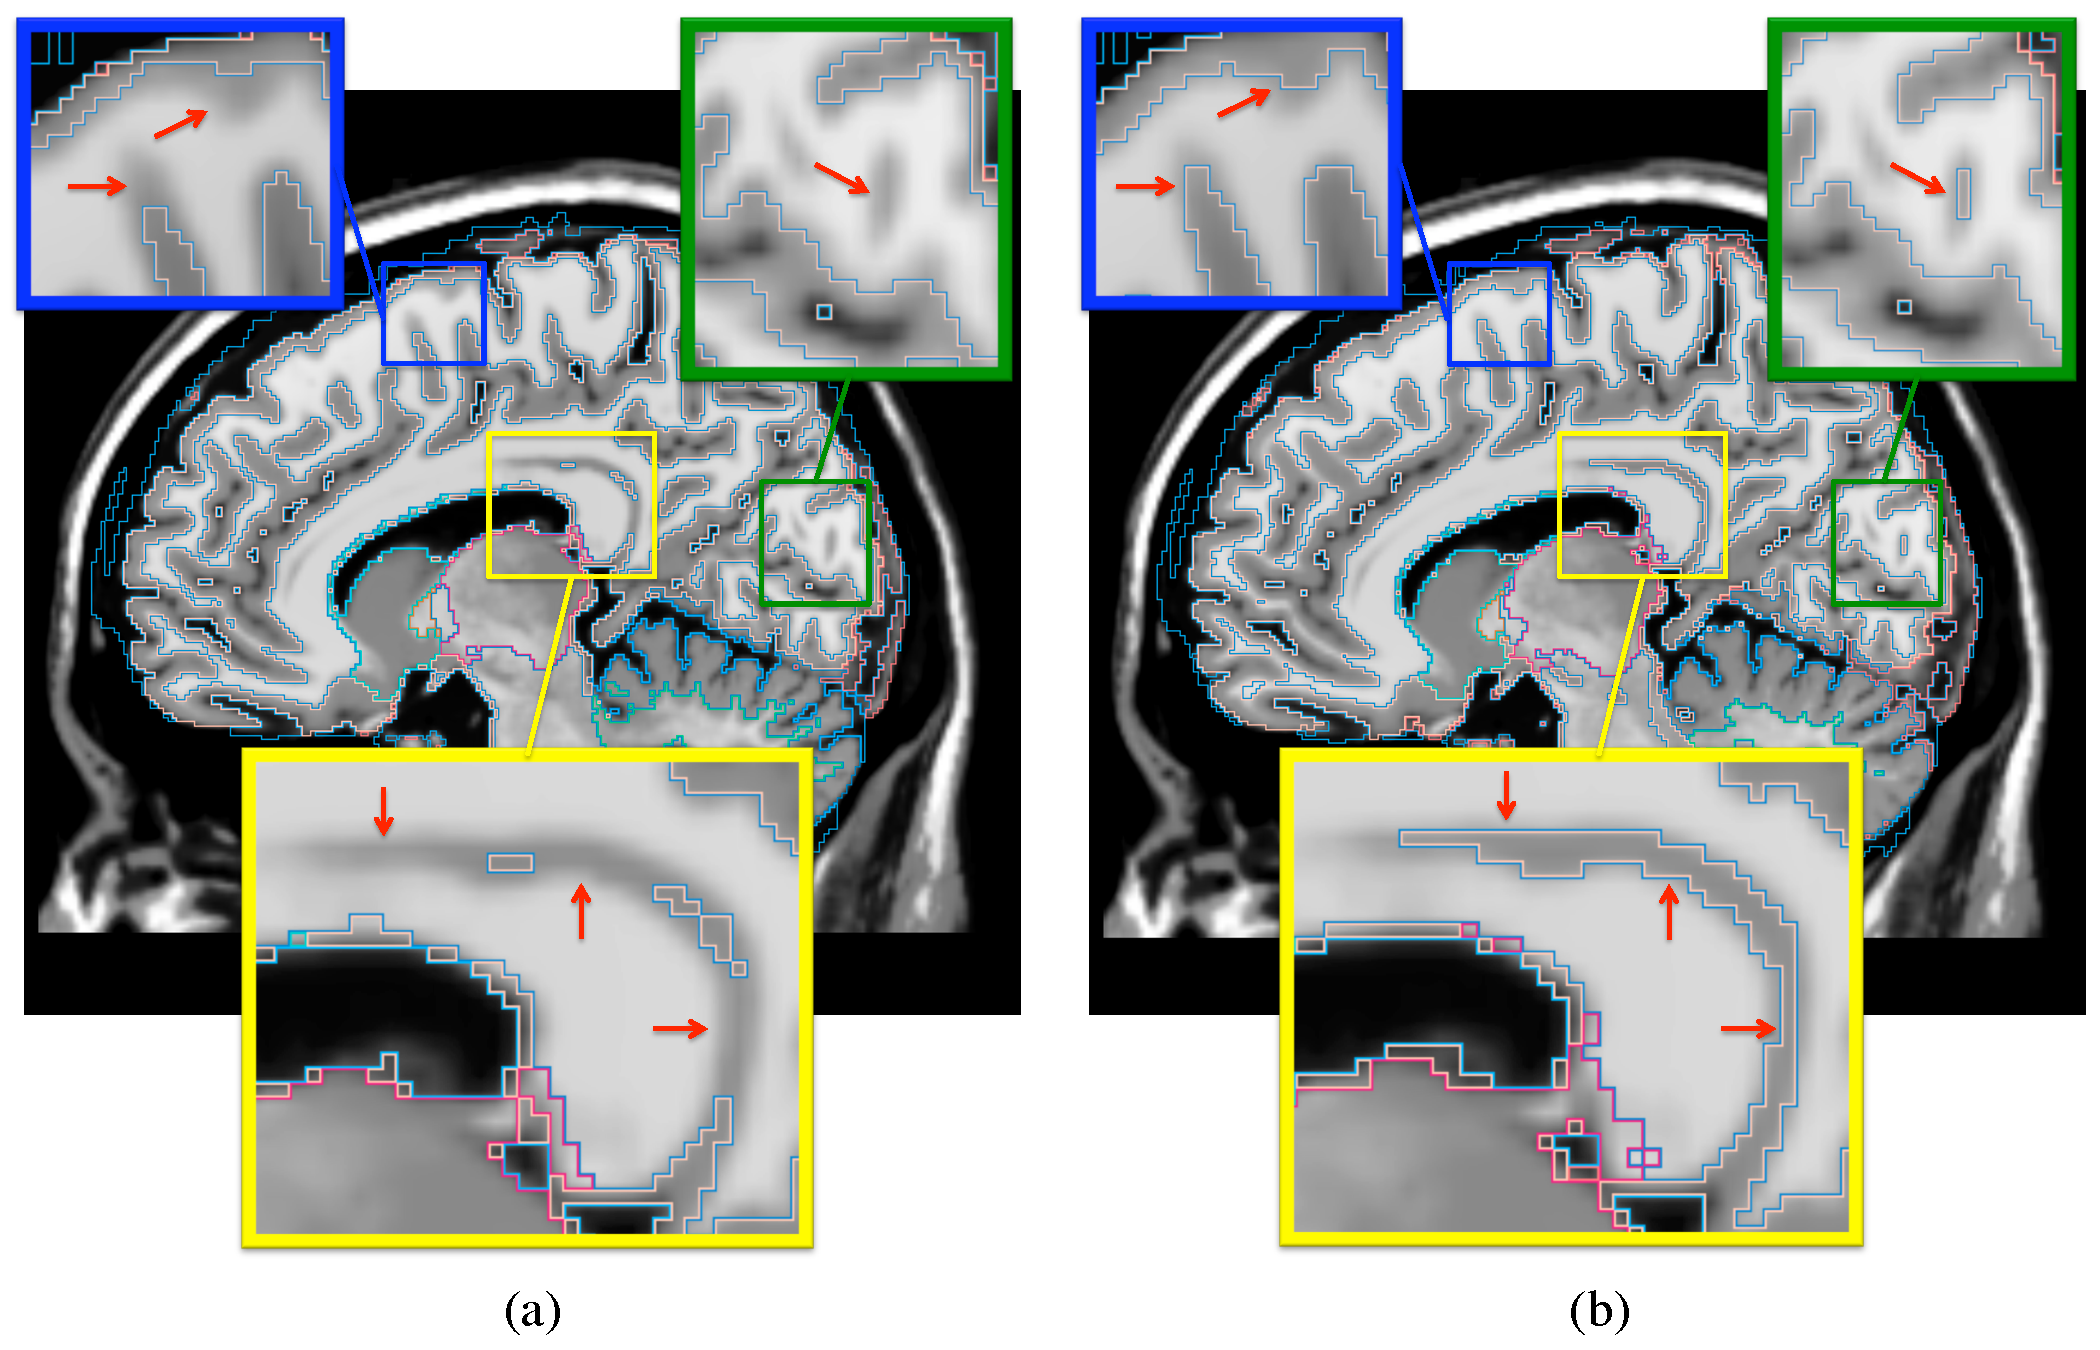
\includegraphics[width=6.4in,height=4.1in]{UsePurePlugs_qualitative}\
\centering
\caption{(a) Segmentation results when pure plugs mask is not incorporated in classifiction process. (b) Results when only pure samples are used to initialize/train the classification methods. Incorporating pure samples in the classification process enhances segmentation in tissue boundaries and can help detecting missed subtle tissue regions.}
\label{fig:UsePurePlugs_qualitative}
\end{figure}
%--------------------------------

\subparagraph{Quantitative Evaluation} %-----------------

Proposed enhancements were evaluated quantitatively using BrainWeb database as described in section \ref{brainWebData}.

Four experiments are run to present the results in Figure (\ref{fig:Use_pure_plugs}). \textit{Green} color shows the results when two modalities are used ($T1$ and $T2$), and both images have the same isotropic $1$ $mm^3$ voxel lattice. 
\textit{Blue} color shows results when two modalities with different resolutions are used. $T1$ is $1 \times 1 \times 1$ $mm^3$, but $T2$ has the voxel sizes as $1 \times 1 \times 3$ $mm^3$.
In both cases, solid lines show the segmentation results when pure plugs mask is \textit{NOT} used, while dashed lines show segmentation results when pure plugs are computed and incorporated to the segmentation process.

%--------------------------------
\begin{figure}
\centering
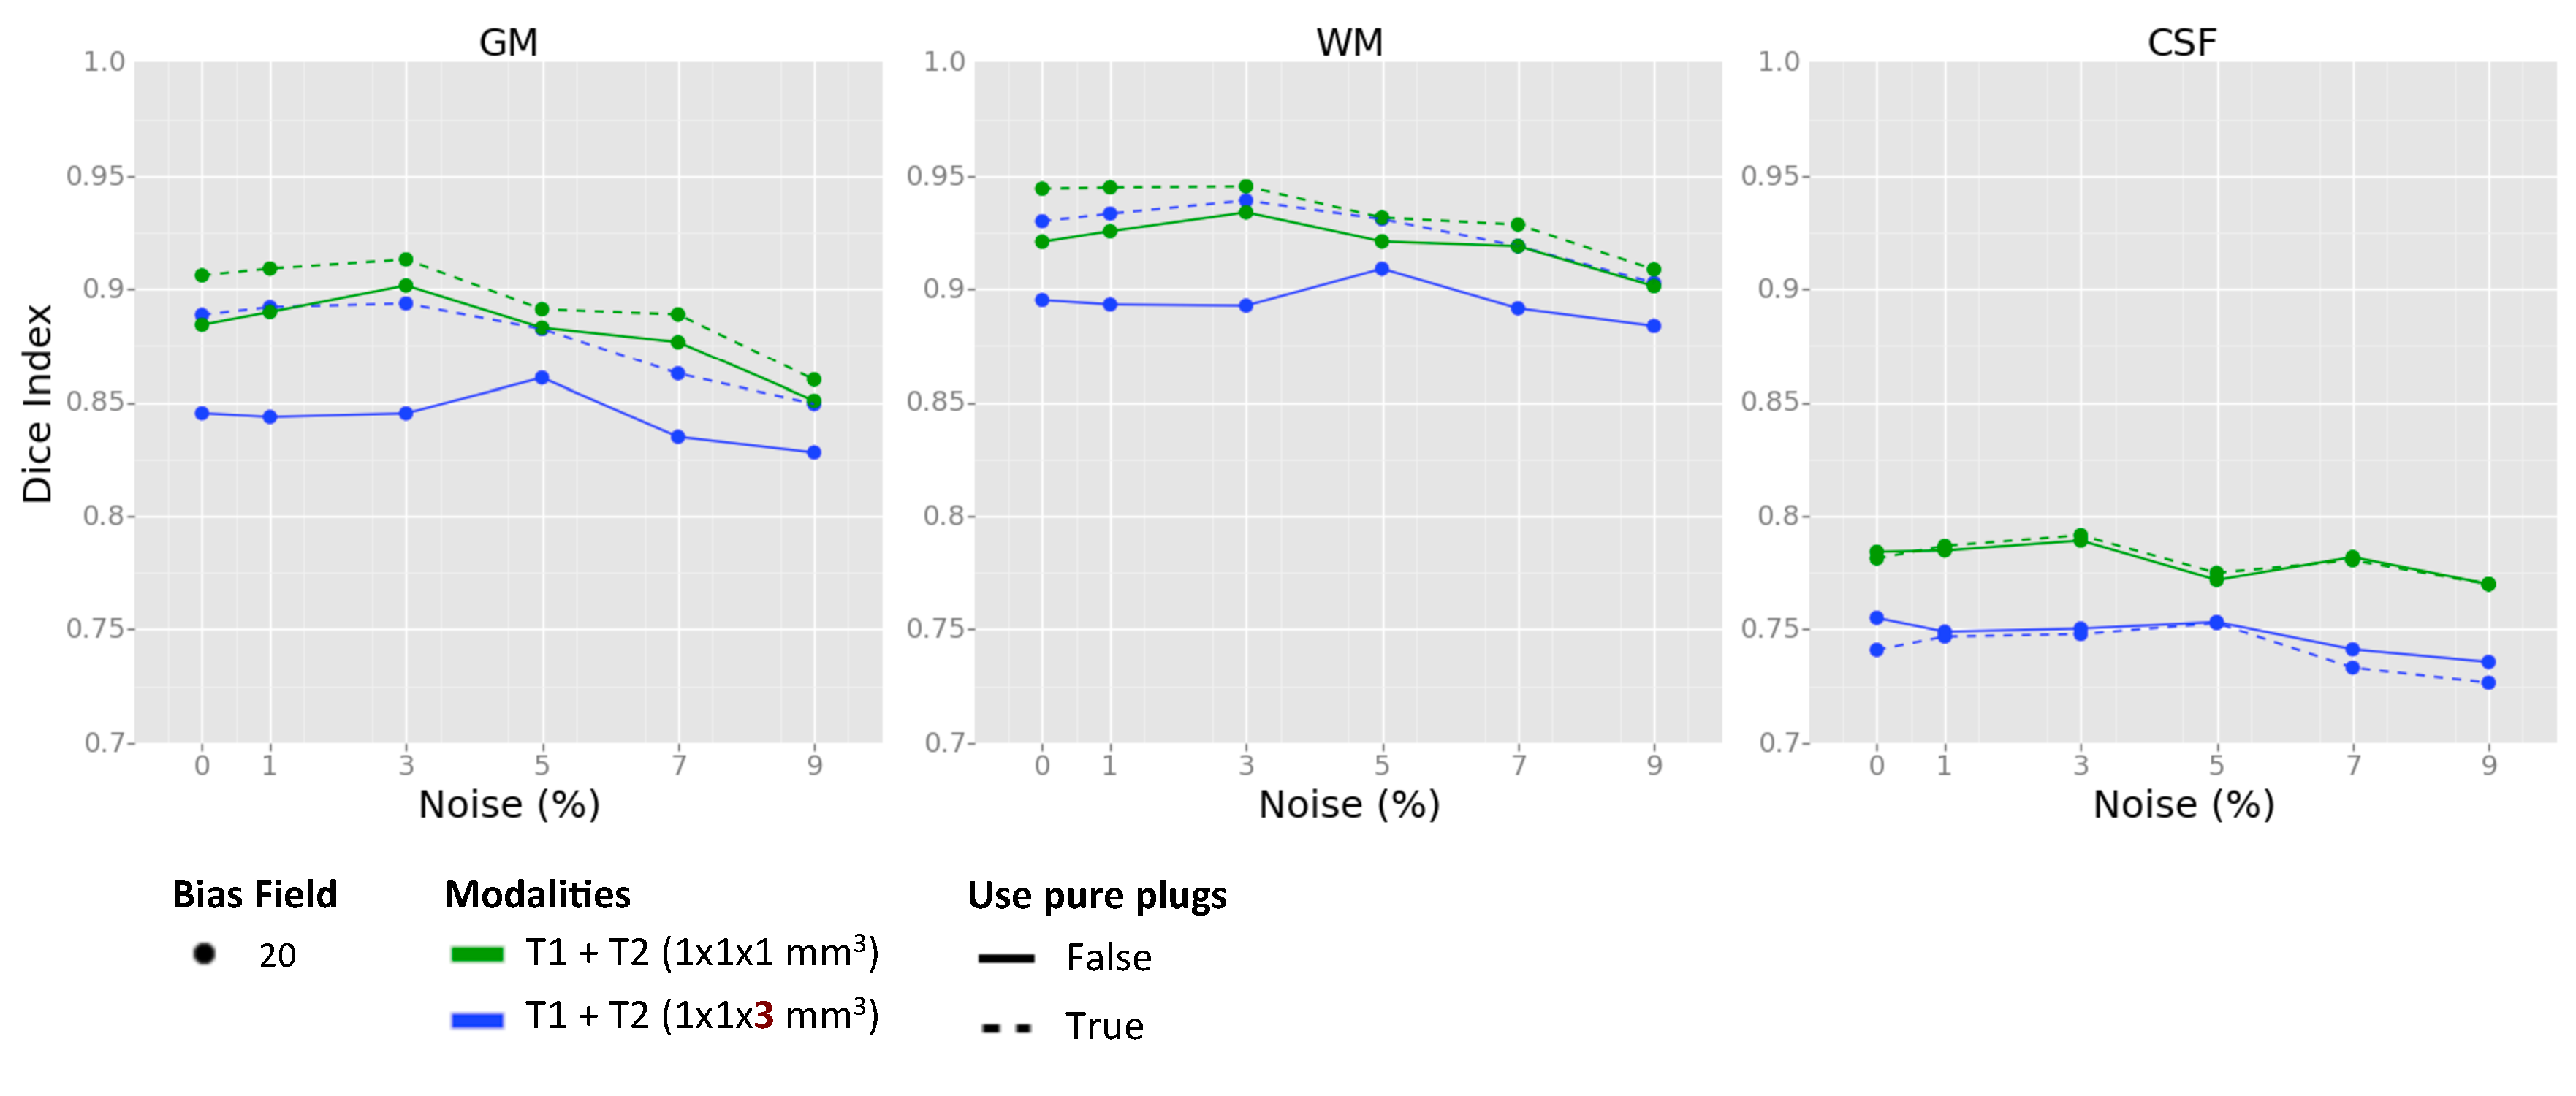
\includegraphics[width=7.6in,height=3.3in]{Use_pure_plugs}\
\centering
\caption{Green lines show the results when the multi-modal segmentation is run using two modalities with the same isotropic $1$ $mm^3$ resolution. Dashed lines show the improved results when only pure samples are involved in the classification process. This improvement is more significant when the second modality has lower spatial resolution as indicated by blue lines.} 
\label{fig:Use_pure_plugs}
\end{figure}
%--------------------------------
 
\paragraph{Discussion and Conclusions}

Results show that considering pure plugs in classification always enhances the results for GM and WM, such that multimodal classification with low resolution T2 and using pure plugs mask outperforms the situation when high resolution T2 is added and pure plugs are not used.

For CSF, Adding pure plugs does not cause any significant changes to the results. It can be because of following reason:
\begin{itemize}
    \item[-] In the ground truth, CSF is manually identified only from T1 modality; however, T1 does not provide enough information to label CSF accurately.
    \item[-] Proposed method is expected to show big difference when regions are highly interleaved together like WM and GM; however, CSF is large pool areas in ventricles and borders of brain.
\end{itemize}


\subsubsection{Research Design for Aim 1 Subtask 3: Extract geometric mean of diffusion images from DWI data, and use these low-resolution information for further enhancement of tissue classification}
\label{section:Aim1Subtask3ResearchDesign} %--------------------

In this section we propose further potential enhancements to the segmentation results by adding complementary information from diffusion properties, derived from the diffusion-weighted imaging (DWI) data, to the classification process.

\paragraph{Significance}

Adding $T2$-weighted MR modality caused better classification for CSF, and Blood Venous, since $T2$ provides better contrast for CSF versus Bone Marrow, and for Blood Venous versus Gray matter.

Diffusion data, extracted from diffusion-weighted imaging (DWI) modality, provides valuable information about characterization of the brain white matter architecture; therefore, by adding them to the classification process, we expect to get better WM/GM classification.

\paragraph{Approach}

We propose following approach for furthur potential improvements in tissue classification results:
\begin{itemize}
    \item First, isotropic diffusion-weighted information (IDWI), that is the geometric mean of the diffusion images, is extracted from diffusion-weighted imaging ($DWI$) dataset. Figure (\ref{fig:sample_IDWI}) shows the mid-slice views of a $3D$ $IDWI$ image extracted from the $4$-dimensional $DWI$ modality from a test subject image listed in Table (\ref{PurePlugsMaskTestData}).
    \item The extracted $IDWI$ image is then incorporated into the classification process as a new modality channel.
\end{itemize}

%--------------------------------
\begin{figure}
\centering
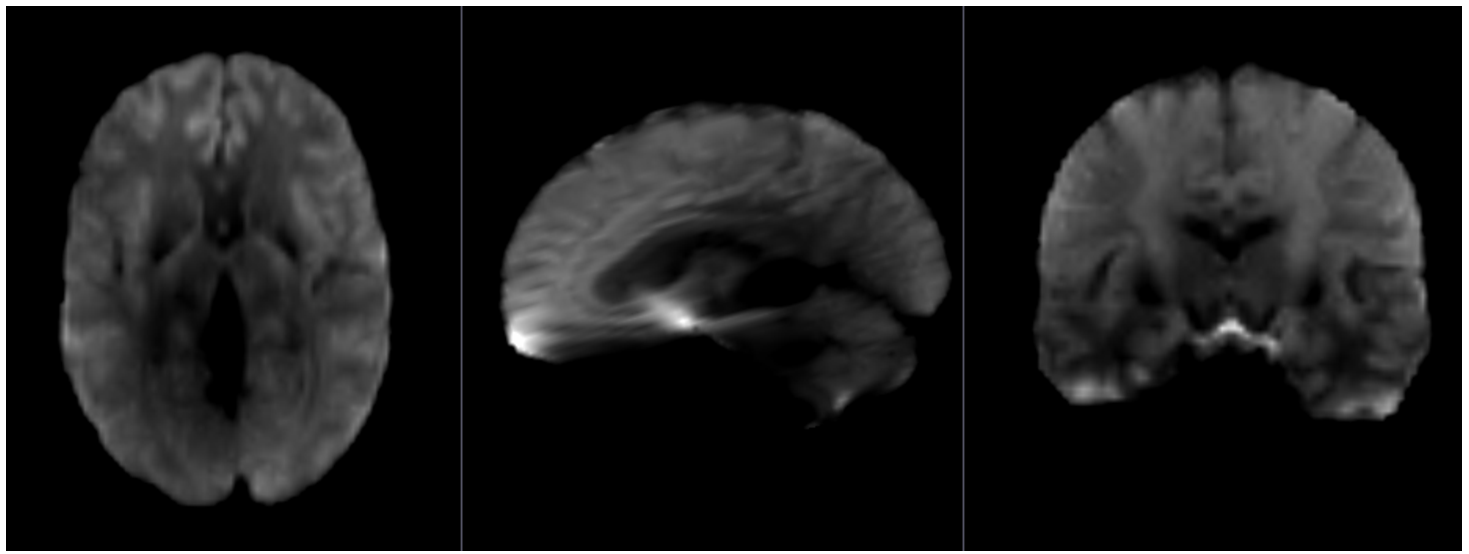
\includegraphics[width=5.5in,height=2in]{sample_IDWI}\
\centering
\caption{Mid-slice views of a sample $3D$ IDWI image extracted from a $4D$ diffusion-wighted imaging modality from a subject test listed in table (\ref{PurePlugsMaskTestData}). IDWI is the geometric mean of all diffusion images in a DWI dataset.} 
\label{fig:sample_IDWI}
\end{figure}
%--------------------------------

\paragraph{Evaluation}

In Aim 1 - subtask 2, the proposed method showed enhancements to the segmentation results by using low-resolution $T2$ data with voxel sizes $3$ times larger than the $T1$ data.
Here we propose to investigate the effectiveness of that method when we add a new modality source with significantly lower spatial resolution, where each cubic voxel is $8$ times larger than the high-resolution $T1$ voxels.

\subparagraph{Test Data}

Five imaging datasets from the human brain will be selected from the PREDICT-HD database, such that they are taken at one time point from $5$ different subjects and are collected from $5$ different sites. Each dataset will include three different MR modalities of $T1$-weighted, $T2$-weighted and diffusion-weighted imaging (DWI) scans, where $T1$ and $T2$ are provided in higher spatial resolution of $1$ $mm^3$, but $DWI$ data are acquired in a very low spatial resolution of $2 \times 2 \times 2$ $mm^3$.

\subparagraph{Experimental methods}

In this regard, we propose:
\begin{itemize}
    \item[-] Use $3D$ Slicer \cite{slicer_paper} to manually label $WM$, $GM$, and $CSF$ tissue regions in the mid-axial slice of each test dataset. This information will be used as a baseline to evaluate the segmentation results.
    \item[-] Run multi-modal segmentation on selected datasets, first, using two $T1$ and $T2$ modalities, and then using $3$ MR modalities ($T1$, $T2$, and $IDWI$) with and without using pure plugs mask.
    
    ``Dice Index'' and ``Hausdorff distance'' will then be used as the similarity measures to compare the results of each segmentation experiment with manually provided ground truth.
\end{itemize}

\subsubsection{Expected Results}

Diffusion information provides a new source to distinguish between the White matter and Gray matter structures as shown by Figure (\ref{fig:sample_IDWI}). This information can help us to increase the interpretability of our data by generating a better segmentation in White matte and Gray matter tissue boundaries. This will guide a better estimate of cortical thickness that is a critical factor in neurodegenerative studies.
\newline

\subsubsection{Potential Problems}

The classification framework enhanced by the method proposed in Aim 1 - Subtask 2 was evaluated using two input modalities where the resolution of the second modality is $3$ times lower than the first modality scan. However, the voxel size of a typical $IDWI$ image is $2 \times 2 \times 2$  $mm^3$, which is $8$ times bigger than a conventional $T1$-weighted $MR$ scan. Therefore, the framework provided in Aim 1 - Subtask 2 may need to be tuned with a new set of parameters to efficiently deal with larger partial volume effect and to work best with more than two input modality channels.
\newline

\subsubsection{Status}
\begin{itemize}
    \item The method in Aim 1 - Subtask 1 has been developed and evaluated on the BrainWeb dataset explained in section \ref{brainWebData}. More thorough discussion of the methods and results have been published in:
    \begin{itemize}
        \item[-] {A.~Ghayoor}, J.~S.~Paulsen, R.~E.~Kim, and H.~J.~Johnson, ``Tissue classification of large-scale multi-site MR data using fuzzy k-nearest neighbor method,'' In \textit{SPIE Med. Imag. 2016: Image Processing}, 9784, 9784–66 (7 pages). 
    \end{itemize}
    
    \item The method in Aim 1 - Subtask 2 has been developed and evaluated on the BrainWeb dataset. Also, it contributed to a fully automated $MR$ processing pipeline for the PREDICT-HD study. It helped to take the advantage of the low-resolution $T2$-weighted $MR$ images acquired from $1.5$ Tesla scanners in the classification process. These data were ignored in previous runs of the processing pipeline, since they were adversely affecting the segmentation results due to the issues caused by the partial volume effect.
    
    \item The approach proposed in Aim 1 - Subtask 3 is under development.
    
    \item The proposed method and the evaluation results will be submitted as a paper to frontiers in neuroscience journal.
\end{itemize}

%===============================================================
%===============================================================
%===============================================================
%===============================================================
%===============================================================
\subsection{Aim 2: Super-resolution reconstruction of low-resolution diffusion-weighted imaging data using a \emph{priori} knowledge of underlying anatomical structure}
\label{subsection:Aim2ResearchDesign}

\subsubsection{Significance}

Diffusion-weighted imaging (DWI) is a key imaging modality that enables non-invasive and in-vivo investigation and characterization of brain white matter architecture and microstructure and is widely applied in neurological applications.

DWI is, however, strongly limited by its relatively low spatial resolution. The resolution of current typical DWI data is $2 \times 2 \times 2$  $mm^3$, that means its voxel is $8$ times larger than that in structural MRI. 
Increasing the resolution of DWI acquisitions can allow investigation of novel fiber structures and will enable a more accurate assessment of the brain connectivity by tracing small white matter fiber bundles. Also, high resolution images are critical to reduce partial volume effects. 
However, increasing the resolution is challenging in DWI. A DWI scan needs to be repeated 64 times for averaging to increase the resolution from $2 \times 2 \times 2$ $mm^3$ to $1 \times 1 \times 1$ $mm^3$ while keeping the similar signal-to-noise ratio \cite{brown2014}. It means that 5 minute acquisition would become a 5 hour scan, which is not feasible. 

To enhance the resolution, image post-processing methods are an alternative to hardware improvement.
However, simply using the interpolation methods to increase the resolution causes results show blurry edges.
The term of super-resolution reconstruction (SRR) refers to considering image degradation process to estimate the latent high resolution image from the input low resolution.

%There are only few studies on SRR methods for DWI. 
To overcome the limitations of low-resolution DWI, some SRR methods have been recently developed.
%Existing techniques can be classified into two general categories based on their data acquisition techniques. The first
One group of methods require multiple low-resolution (LR) images to reconstruct a high-resolution (HR) image.
%
Scherrer \emph{et al.} \cite{scherrer2012} suggested to acquire multiple anisotropic orthogonal DWI scans and fuse them into a high resolution output.
%
Ning \emph{et al.} \cite{ning2015} combined the concept of compressed sensing and classical super-resolution to reconstruct high-resolution DWI from multiple sub-pixel-shifted thick-slice LR acquisitions with non-overlapping diffusion directions to reduce acquisition time.
%
However, these types of methods are hampered for general applications because: first, a specially designed image acquisition method is needed to acquire multiple scans; second, the subject motion and eddy current effects in different scans could largely affect the final results.
%
The other group of methods obtain HR data using a single LR image through a learning process or an intelligent regularization.
%
Alexander \emph{et al.} \cite{alexander2014} proposed a method to exploit information from expensive high quality datasets and transfer them to enhance the images acquired from a more modest data acquisition. Their method attempts to learn mapping from LR to HR through training sets using patch-based image representation and random forest regression. Tarquino \emph{et al.} \cite{tarquino2014} suggested a patch-based sparse representation approach to recover HR reconstruction using the coupled low and high resolution dictionaries. Although these methods do not require multiple LR acquisition, they still need a separate HR training dataset.
% for Alexander et al:
% - In their method they have proposed to exploit information in expensive high quality data sets to improve images reconstructed from more modest data acquisitions (In this aspect it is kind of similar to my work). However, in following aspects it is different than my method:
% - Their method attempts to learn mapping from low resolution to high resolution through training sets using patch-based image representation and random forest regression. In their implementation, they have used randomly selected high resolution DWI data from Human Connectome Porject (HCP) as the training data set. In fact, their method does not use multi modal information but needs a separate training data set.
% - Also, their implementation presented to operate directly on Diffusion Tensor Images (DTI) rather than raw DWI data.
Shi \emph{et al.} \cite{shi2015} proposed a method for super-resolution reconstruction of a single LR scan by modeling degradation process and use of different regularization terms. However, the performance of their method still largely relies on the information contained in the original LR image.

Here, we propose a novel method for super-resolution reconstruction of input DWI image using the prior anatomical information extracted from other modality sources provided in higher spatial resolution.
Particularly, we incorporate the brain anatomy description provided by high-resolution structural MR (T1/T2-wighted) scans into super-resolution reconstruction of DWI image.
Our method aims to increase the resolution of the input low-resolution DWI to a high-resolution DWI, e.g., at a factor of 2. Our contribution is two fold: 1) Create a combined edge map from the structural MR scans in higher spatial resolution ($1 \times 1 \times 1$ $mm^3$); 2) Use the created edge map as discrete spatial weights in a weighted total variation (WTV) method.
\newline

\subsubsection{Mathematical Background} %----------------

\paragraph{Regularized recovery of inverse problems} %-----------

Image reconstruction is the process of the recovery of an ideal intensity image from its corrupted or indirect measurements. Such a process is considered as an inverse problem in science as it starts with the results (observations) and then calculates the causes. The observed data are usually related to the ideal, unknown image through a ``forward'' transformation \cite{geman95}.

We consider the recovery of a continuously differentiable image $f:\Omega \rightarrow \mathbb{R}$ from its measurements $b$. Here, $\Omega \subset \left \{ \mathbb{R}^{n} \mid n = 2 \quad or \quad 3 \right \}$ is the spatial support of the image. The acquisition scheme is modeled by the linear operator $\mathcal{A}$, i.e.,

\begin{equation}
\begin{gathered}
b = \mathcal{A}(f) + n
\end{gathered}
\end{equation}

Where $n$ is assumed to be a Gaussian distributed white noise with standard deviation of $\sigma$.

The recovery is ill posed in many practical applications as the operator $\mathcal{A}$ is ill conditioned. One popular approach is to add a regularization penalty to the inverse problem.
Regularization is a method for adding constrains, from some a \emph{priori} information or assumption about the structure of $f$, in addition to those implicit in coherence to the data.
By formulating the minimization problem using Lagrange multipliers:

\begin{equation}
\label{eq:nonweightedregularization}
\begin{gathered}
\widehat{f} = arg\min_{f}\left\|\mathcal{A}(f)-b\right\|^{2} + \lambda\mathcal{J}(f)
\end{gathered}
\end{equation}

%\mathscr{F}

Where the first term ensures fidelity to the data, and the second term imposes a roughness regularization penalty $\mathcal{J}$ that is a convex functional of $f$.
The optimal parameter $\lambda$ is a positive parameter that balances theses two terms and is chosen such that $\left\|\mathcal{A}(\hat{f})-b\right\|^{2} \approx \sigma^{2}$.

One popular choice for the regularization term includes quadratic penalties \cite{tikhonov1943stability} that is the squared $l_{2}$ norm of either the image $f$ or its (discrete) derivatives:

\begin{equation}
\begin{gathered}
\mathcal{J}(f) = \left\|\triangledown f\right\|^{2} = \int_{\Omega} |\triangledown f|^2 d\Omega
\end{gathered}
\end{equation}

Above penalty term is well-known as Tikhonov regularization \cite{tikhonov1977solutions}. By using a quadratic regularization term, the estimator $\widehat{f}$ becomes a linear combination of the data values that provides computational advantages. However, quadratic estimators suffer from oversmoothing of the recovered image, as they and do not recover the important attributes of $f$, such as the location and magnitude of jumps, or higher order discontinuities \cite{geman95}. To show this, consider $1-D$ computation on step edges.

\subparagraph{1-D computation on step edges} %----------------
Set $\Omega = [-1,1]$, and $f$ the step edge function:

\begin{equation}
\begin{gathered}
f(x) = 
\left \{
  \begin{tabular}{cc}
  0 & x $\leq$ 0 \\
  a & x $>$ 0
  \end{tabular}
\right.
\end{gathered}
\end{equation}

Where $a$ is a real number. Then, the regularization penalty can be written as:

\begin{equation}
\begin{gathered}
\mathcal{J}(f) = \int_{-1}^{1} \left | {f}'(x) \right |^{2}dx
\end{gathered}
\end{equation}

Although $f$ is not differentiable at $0$, we try to compute the above penalty by approximating ${f}'(x)$ around $0$:

\begin{equation}
\begin{gathered}
{f}'(x) \approx \frac{f(h)-f(-h)}{2h} \approx \frac{a}{2h} \\
\quad s.t. \quad x\in [h,-h] \quad and \quad h>0, small
\end{gathered}
\end{equation}

Then:

\begin{equation}
\begin{gathered}
\int_{-1}^{1} \left | {f}'(x) \right |^{2}dx = \int_{-1}^{-h} \left | {f}'(x) \right |^{2}dx + \int_{-h}^{h} \left | {f}'(x) \right |^{2}dx + \int_{h}^{1} \left | {f}'(x) \right |^{2}dx \\
\approx 0 + 2h \times (\frac{a}{2h})^{2} + 0 \approx \frac{a^2}{2h} \rightarrow \infty, h \rightarrow 0
\end{gathered}
\end{equation}

Therefore, a step-edge is severely penalized as it has infinite energy and cannot minimize the Tikhonov regularization. Now replace the square in previous computations by $p>0$:

\begin{equation}
\label{eq:plessthan1}
\begin{gathered}
\int_{-1}^{1} \left | {f}'(x) \right |^{p}dx \\
\approx 0 + 2h \times |\frac{a}{2h}|^{p} + 0 \approx |a|^{p}(2h)^{1-p} < \infty, \quad when \quad p \leq 1
\end{gathered}
\end{equation}

Equation (\ref{eq:plessthan1}) shows that the regularization term is finite when $p \leq 1$, so edges are less penalized. Note that when $p=1$, this is the ``Total Variation'' of $f$ \cite{rudin1992nonlinear} where the penalty is the $l_{1}$ norm of the gradient magnitude of the signal, i.e.,

\begin{equation}
\begin{gathered}
\mathcal{J}_{TV}(f) = \int_{\Omega} |\triangledown f| d\Omega
\end{gathered}
\end{equation}

The concept of using total variation in image processing was first introduced by Rudin \emph{et al.} \cite{rudin1992nonlinear} for noise removal, since it is very effective at simultaneously preserving edges while smoothing noise in flat regions. In addition, total variation (TV) minimization is widely used for reconstruction of images with sparse gradients that specially makes sense as many natural images have sparse or nearly sparse gradients \cite{blomgren1998color}.

Generally, constrained $l_{1}$ minimization methods are well-known for reconstruction of sparse signals from highly incomplete sets of linear measurements \cite{candes2008enhancing}. This is thoroughly investigated in the next section.

\paragraph{$l_{1}$-norm minimization in sparse signal recovery}

One of the challenging problems in engineering is to reconstruct a signal when there are fewer equations than unknowns. Such a problem of course does not have a unique solution without some additional information. However, we can recover a signal $x_{0}\in \mathbb{R}^{n}$ by solving the following optimization problem under the sparsity assumption, when the unknown signal that we wish to recover depends upon a smaller number of unknown parameters:

\begin{equation}
\label{eq:l0norm}
\begin{gathered}
\min_{x\in \mathbb{R}^{n}}\left\|\Phi x-y\right\|^{2} + \lambda \left \|x  \right \|_{l_{0}}
\end{gathered}
\end{equation}

Where $\Phi$ is an $m \times n$ matrix with fewer rows than columns ($m<n$), and $\left \| x \right \|_{l_{0}}=\left | \left \{ i:x_{i} \neq 0 \right \} \right |$; i.e., number of nonzero samples in $x$.

$l_{0}$ norm is the sparsity count regularization. However, the equation in (\ref{eq:l0norm}) is nonconvex, and a common alternative is to consider the following convex problem:

\begin{equation}
\label{eq:l1norm}
\begin{gathered}
\min_{x\in \mathbb{R}^{n}}\left\|\Phi x-y\right\|^{2} + \lambda \left \|x  \right \|_{l_{1}}
\end{gathered}
\end{equation}

Where $\left \| x \right \|_{l_{1}}=\sum_{i=1}^{n}\left | x_{_{i}} \right |$. In equation (\ref{eq:l1norm}), $l_{1}$ norm is used as a poxy for the $l_{0}$ sparsity count.

\paragraph{Enhance sparsity recovery in $l_{1}$-norm minimization}
\label{section:Enhancel1NormMinimization}

Like $l_{0}$ norm, the $l_{1}$ norm regularization term has an advantage over quadratic penalty functions as it preserves jumps in the function. However, a key difference between the $l_{1}$ and the $l_{0}$ norms is the dependence on magnitude, such that larger coefficients are penalized more heavily than the smaller coefficients in the $l_{1}$ norm. To address this imbalance, Candes \emph{et al.} have suggested a weighted formulation of $l_{1}$ minimization to more democratically penalize nonzero coefficients \cite{candes2008enhancing}:

\begin{equation}
\label{eq:weightedl1norm}
\begin{gathered}
\min_{x\in \mathbb{R}^{n}}\left\|\Phi x-y\right\|^{2} + \lambda \left \|Wx  \right \|_{l_{1}}
\end{gathered}
\end{equation}

Where $\left \| Wx \right \|_{l_{1}}=\sum_{i=1}^{n}w_{i}\left | x_{_{i}} \right |$, and each $w_{i}$ is a positive weight.

In general, weighted and unweighted $l_{1}$ minimization have different solutions, since weights can be considered as free parameters in the convex problem, whose values ``can'' improve the signal reconstruction if they are set wisely.

\subparagraph*{What values for the weights will improve signal reconstruction?}
As a rough rule of thumb, weights should be chosen such that they counteract the influence of the signal magnitude on the $l_{1}$ penalty function. Suppose we know the true signal $x_{0}$; then, the weights can be inversely proportional to the true signal magnitude such that:

\begin{equation}
\label{eq:idealweights}
\begin{gathered}
w_{i} = \left\{\begin{matrix}
\frac{1}{\left | x_{0,i} \right |} , & x_{0,i} \neq 0 , \\ 
\infty , &  x_{0,i} = 0.
\end{matrix}\right.
\end{gathered}
\end{equation}

Ideally, zero-valued components of $x_{0}$ are prohibited in the recovered signal being penalized by large (infinite) entries of $w_{i}$, while the largest signal coefficients are encouraged to be identified as nonzero in the recovered signal being penalized less by small (finite) $w_{i}$ entries. It is of course impossible to construct the precise weights without knowing the true signal $x_{0}$, so a valid set of weights can be designed based on an approximation $\hat{x_{0}}$ to $x_{0}$. Also, To provide stability, the equation (\ref{eq:idealweights}) is rewritten as following by introducing the parameter $\epsilon > 0$:

\begin{equation}
\label{eq:weights}
\begin{gathered}
w_{i} = \frac{1}{\left | \hat{x_{0,i}} \right | + \epsilon } , \quad \epsilon > 0
\end{gathered}
\end{equation}

Where $\epsilon$ should be set slightly smaller than the expected nonzero magnitudes of $\hat{x_{0}}$ \cite{candes2008enhancing}. In addition to stability, using $\epsilon$ ensures that a zero-valued entry in approximated $\hat{x_{0}}$ does not strictly prohibit a nonzero estimate in the recovered signal.

Using above weights in minimization problem (\ref{eq:weightedl1norm}) makes the solution $x$ to concentrate on the large nonzero entries in $x_{0}$ since they will be penalized less by small $w_{i}$ entries, while zero-valued entries on $x_{0}$ will be largely penalized and are discouraged in the recovered signal.

\paragraph{Analytical justification} %------------------------
\label{subsubsection:analyticalJustification}

Using a concave penalty function, instead of the $l_1$-norm regularization term in equation (\ref{eq:l1norm}), more closely resembles the $l_0$-norm regularization. It is illustrated in Figure (\ref{concave_penalty_function}), where the $f_{log,\epsilon}(t)$ is defined as:

\begin{equation}
\label{eq:concaveFunction}
\begin{gathered}
f_{log,\epsilon}(t) = log(1+\frac{\left | t \right |}{\epsilon })
\end{gathered}
\end{equation}

Like the $l_0$ norm, the $f_{log,\epsilon}(t)$ allows a relatively large penalty to be placed on small nonzero coefficients. In fact, $f_{log,\epsilon}(t)$ tends to $f_0(t)$ as $\epsilon \rightarrow 0$.

%--------------------------------
\begin{figure}
\centering
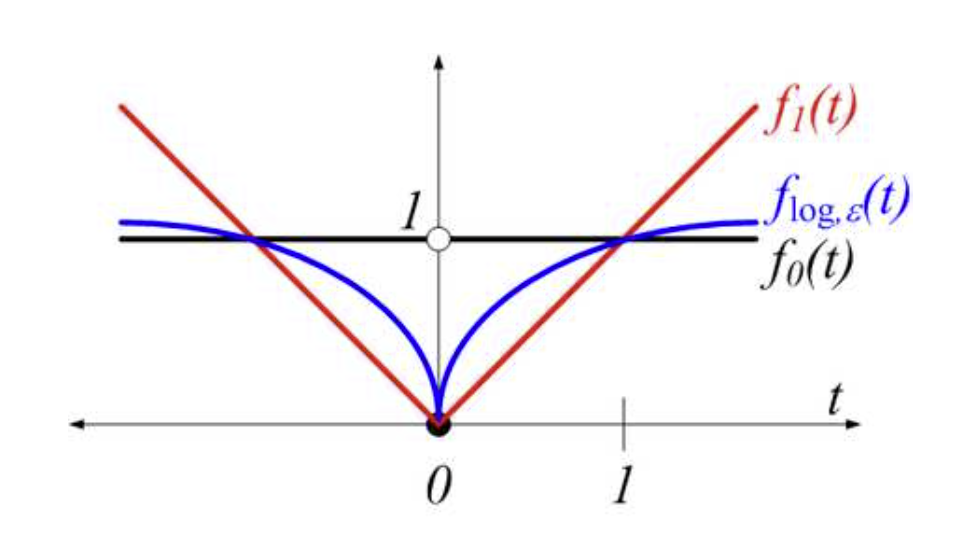
\includegraphics[width=3.5in,height=1.75in]{concave_penalty_function}\
\centering
\caption{The log-sum concave penalty function $f_{log,\epsilon}(t)$ is a better approximation for the $l_0$ sparsity count $f_0(t)$ rather than the traditional convex $l_1$ regularization $f_1(t)$ \cite{candes2008enhancing}.}
\label{concave_penalty_function}
\end{figure}
%--------------------------------

In this section, we show that using a weighted $l_{1}$ minimization of as weights defined in (\ref{eq:weights}) is like to find the local minimum of a concave penalty function as defined in (\ref{eq:concaveFunction}). 

To establish this connection, consider the following problem:

\begin{equation}
\begin{gathered}
\min_{x\in \mathbb{R}^{n}}\left\|\Phi x-y\right\|^{2} + \lambda \sum_{i=1}^{n} log(1+\frac{\left | x_{i} \right |}{\epsilon })
\end{gathered}
\end{equation}

Which is equivalent to 

\begin{equation}
\label{eq:log}
\begin{gathered}
\min_{x\in \mathbb{R}^{n}} 
\sum_{i=1}^{n} log(1+\frac{\left | x_{i} \right |}{\epsilon })
\quad subject \quad to \quad y=\Phi x
\end{gathered}
\end{equation}

Above optimization problem can be solved using a majorize-minimize (MM) \cite{hunter2004} framework by iteratively minimizing a simple surrogate function majorizing a given objective function, so (\ref{eq:log}) is equivalent to:

\begin{equation}
\label{eq:logsurrogate}
\begin{gathered}
\min_{x,u\in \mathbb{R}^{n}} 
\sum_{i=1}^{n} log(1+\frac{u_{i}}{\epsilon })
\quad subject \quad to \quad \begin{matrix}
y=\Phi x,\\
\left | x_{i} \right | \leq u_{i}, i=1,..,n. 
\end{matrix}
\end{gathered}
\end{equation}

If $\hat{x}$ is a solution to (\ref{eq:log}), then $(\hat{x},\left | \hat{x}  \right |)$ is a solution to (\ref{eq:logsurrogate}). Also, conversely, if $(\hat{x},\hat{u})$ is a solution to (\ref{eq:logsurrogate}), then $\hat{x}$ is a solution to (\ref{eq:log}). Now, set:

\begin{equation}
\label{eq:funcg}
\begin{gathered}
g\left ( u \right ) =
\sum_{i=1}^{n} log(1+\frac{u_{i}}{\epsilon })
\end{gathered}
\end{equation}

Function $g$ is concave and below its tangent, so it can be minimized by iteratively improving on an initial guess $u^{\left ( 0 \right )}$.
At each iteration, we minimize a linear approximation of $g$ around the previous guess $u^{\left ( l \right )}$ derived from the first-order Taylor polynomial:

\begin{equation}
\begin{gathered}
u^{\left ( l+1 \right )} = arg \min\left \{ g\left ( u^{\left ( l \right )} \right ) + \bigtriangledown g\left ( u^{\left ( l \right )} \right ).\left ( u-u^{\left ( l \right )} \right ) \right \} 
\quad subject \quad to \quad u\in \mathcal{C}
\end{gathered}
\end{equation}

Where $\mathcal{C}$ is a convex set. Each iteration of above problem is a convex optimization problem, since it is minimization of a linearization of $g$ around previous guess:

\begin{equation}
\begin{gathered}
u^{\left ( l+1 \right )} = arg \min \bigtriangledown g\left ( u^{\left ( l \right )} \right ).u
\quad subject \quad to \quad u\in \mathcal{C}
\end{gathered}
\end{equation}

In the case of optimization problem in (\ref{eq:logsurrogate}), this gives:

\begin{equation}
\begin{gathered}
\left ( x^{\left ( l+1 \right )}, u^{\left ( l+1 \right )} \right ) =
arg \min \sum_{i=1}^{n}\frac{u_{i}}{u_{i}^{\left ( l \right )}+\epsilon }
\quad subject \quad to \quad \begin{matrix}
y=\Phi x,\\
\left | x_{i} \right | \leq u_{i}, i=1,..,n. 
\end{matrix}
\end{gathered}
\end{equation}

Which is equivalent to:

\begin{equation}
\label{eq:mmsolution}
\begin{gathered}
 x^{\left ( l+1 \right )} = arg \min \sum_{i=1}^{n} \frac{\left | x_{i} \right |}{\left | x_{i}^{\left ( l \right )} \right |+\epsilon }
\quad subject \quad to \quad y=\Phi x
\end{gathered}
\end{equation}

By setting:

\begin{equation}
\begin{gathered}
W_{i}^{\left ( l+1 \right )}  = \frac{1}{\left | x_{i}^{\left ( l \right )} \right |+\epsilon }
\end{gathered}
\end{equation}

Then (\ref{eq:mmsolution}) can be rewritten as:

\begin{equation}
\begin{gathered}
x^{\left ( l+1 \right )} = arg \min \sum_{i=1}^{n} W_{i}^{\left ( l+1 \right )} \left | x_{i} \right |
\quad subject \quad to \quad y=\Phi x
\end{gathered}
\end{equation}

That is equivalent to:

\begin{equation}
\begin{gathered}
x^{\left ( l+1 \right )} = arg \min \left \| \Phi x-y \right \|^{2} + \lambda \left \| W^{\left ( l+1 \right )} x \right \|_{l_{1}}
\end{gathered}
\end{equation}

Above is an iterative reweighted $l_{1}$ minimization approach suggested by Candes \emph{et al.} \cite{candes2008enhancing}, in which, each iteration of the algorithm solves a convex optimization problem, whereas the overall algorithm finds a local minimum of a concave penalty function.

If we suppose weights are pre-specified by a ``true knowledge'' of signal $x_{0}$; then, only one iteration of above algorithm would be enough:

\begin{equation}
\label{eq:firstWeightingSolution}
\begin{gathered}
\hat{x_{0}} = arg \min \left \| \Phi x-y \right \|^{2} + \lambda \left \| Wx \right \|_{l_{1}}, \\
\quad where \quad W = \frac{1}{\left | x_{0} \right |+\epsilon }
\end{gathered}
\end{equation}

\paragraph{Variation of weights} %----------------------------

Non-convex regularization terms give reconstruction with less blurring than convex metrics \cite{yang2013}. As shown in section \ref{subsubsection:analyticalJustification}, using pre-specified weights in a weighted $l_1$ minimization is like to find the local minimum of a concave penalty function that is a better approximation of the $l_0$ norm (see Figure (\ref{concave_penalty_function})).

Depending on selected concave function, there are a variety of possible weighting functions in place of $W$ as defined in (\ref{eq:firstWeightingSolution}). For example if instead of a log-sum penalty function, as defined in (\ref{eq:funcg}), we consider an arctangent concave function:

\begin{equation}
\label{eq:atan}
\begin{gathered}
g\left ( u \right ) =
\sum_{i=1}^{n} atan(\frac{u_{i}}{\epsilon })
\end{gathered}
\end{equation}

We can find an alternative formulation of the spatial weights by following the same procedure described in section \ref{subsubsection:analyticalJustification}:

\begin{equation}
\label{eq:newWeights}
\begin{gathered}
W = \frac{1}{ x_{0}^{2}+\epsilon^{2} }
\end{gathered}
\end{equation}

The choice of different variations of the weighting function can be the subject of further empirical studies. The preliminary results of this study are provided based on the choice of weighting function as defined in (\ref{eq:firstWeightingSolution}).
\newline

\subsubsection{Approach}

\paragraph{Weighted total variation minimization for image reconstruction}

To achieve equation (\ref{eq:firstWeightingSolution}), we supposed that we have a true knowledge of signal $x_{0}$. Surprisingly it can be a valid assumption in medical imaging since we may have different representations of the current subject image through different modality sources, where the other modality scans may provide a better estimate of some anatomical features that we wish to recover in the current subject image.

The weighted $l_{1}$ minimization concept, introduced in section \ref{section:Enhancel1NormMinimization}, can also enhance the performance of total-variation (TV) minimization in image reconstruction, since TV can be considered as an $l_{1}$ minimization problem. Weighted-TV problem can then be presented as:

\begin{equation}
\label{eq:weightedregularization}
\begin{gathered}
\widehat{f} = arg\min_{f}\left\|\mathcal{A}(f)-b\right\|^{2} + \lambda \left \| W \left | \bigtriangledown f \right | \right \|_{l_{1}}, \\
\quad where \quad W = \frac{1}{\left | \bigtriangledown \widehat{f_{0}} \right |+\epsilon }
\end{gathered}
\end{equation}

Where $\mathcal{A}$ is a Fourier undersampling operator modeling the physical process that causes degradation; $b$ is the obeservation samples presented as a vector of noisy low-pass Fourier measurements, and $\left | \bigtriangledown f \right |$ denotes the magnitude of the discrete gradients of $f$.

Also, $\left | \bigtriangledown \widehat{f_{0}} \right |$ is an estimation of the gradient magnitude of $f$ computed as an prior edge map from the high resolution representation of the input image subject in other modality scans. 
The spatial weights ($W$) are then constructed from this estimated edge map.

Weights are inversely proportional to the estimation of the gradient magnitude of the input image, such that the most strong edges get the lowest weight values close to zero, and weak edges get higher weights. The maximum weight value is assigned to the smooth regions with no edges.

Some methods have been developed for accurate estimation of the spatial weights. 
Candes \emph{et al.} \cite{candes2008enhancing} suggested an iterative framework to estimate the weights iteratively from the gradient magnitude of the input low-resolution image. First, all weights are set to one; then, at each iteration weights are updated based on the gradient magnitude of the estimated high-resolution image in previous iteration.
Jacob and Ongie \cite{ongie2015} suggested to expand the theory of sampling signals of finite rate of innovation (FRI) on the input low-resolution image to estimate a resolution-independent mask whose zeros represent the edges of the image; then, the spatial weights are created by discretizing the estimated mask at desired resolution.

Here, we propose to create the spatial weights based on a high-resolution edge map estimated from equivalent representation of the underlying anatomical structures in other modality sources.
%Here, we propose to create the spatial weights from an high-resolution edge map estimated from the anatomy description provided by high-resolution representation of the input subject image in other modality sources.
Following section describes the suggested multi-modal framework to estimate a combined edge map from different modality scans provided in higher spatial resolution. Then, spatial weights are constructed from the estimated map as in the equation (\ref{eq:weightedregularization}).

\paragraph{Construction of weights from the estimated anatomical edge map}
\label{section:estimateLabelMap}

Here we describe a multimodal framework to estimate a combined edge map from different modality scans that are equivalent representations of a same underlying anatomical structure. Once the edge map is estimated, the spatial weights are created to be inversely proportional to the edge values.

Assume $I_{i}, i\in \left \{ 1,...,N \right \}$ are different modality scans all representing a single subject image. The gradient of each image is defined as:

\begin{equation}
\label{eq:gradient}
\begin{gathered}
\forall x=(x_{1}, ..., x_{n})\in \left\{voxel \quad locations\right\}, \\
g_{i}(x) = \triangledown I_{i}(x) = \begin{bmatrix}
\frac{\partial I_{i}}{\partial x_{1}}(x_{1}, ..., x_{n}) \\ 
.\\ 
.\\ 
.\\ 
\frac{\partial I_{i}}{\partial x_{n}}(x_{1}, ..., x_{n})
\end{bmatrix}
\end{gathered}
\end{equation}

Where $g_{i}(x)$ is the gradient of the $i^{th}$ input scan at voxel location $x$.
Consequently, the gradient magnitude of each image is defined as:

\begin{equation}
\label{eq:gradientMagnitude}
\begin{gathered}
\left | g_{i}(x) \right | = \left \| \triangledown I_{i}(x) \right \|_{2} = \sqrt{ (\frac{\partial I_{i}}{\partial x_{1}}(x_{1}, ..., x_{n}))^{2} + ... + (\frac{\partial I_{i}}{\partial x_{n}}(x_{1}, ..., x_{n}))^{2} }
\end{gathered}
\end{equation}

Then, the edge map of the underlying anatomical structure is inferred from gradient magnitudes of all input multimodal scans:

\begin{equation}
\label{eq:edgemap}
\begin{gathered}
\forall x\in \left\{voxel \quad locations\right\}, \\
\mu (x) = 
\max_{x}
\left \{ T_{i}\left [ g_{i}(x) \right ] \right \}
\end{gathered}
\end{equation}

Where $T_{i}$ is an image intensity transformation function defined as:

\begin{equation}
\label{eq:intensityTransformFunc}
\begin{gathered}
T_{i}(I) = \begin{cases}
\alpha_{i} I + b_{i} & \text{ if   } Q_I(50) < I < Q_I(95) \\ 
M & \text{ if } I > Q_I(95) \\ 
\epsilon  & \text{ if } I < Q_I(50) 
\end{cases} \\
\quad where \quad \alpha_{i} = \frac{M-\epsilon }{Q_{I}(95)-Q_{I}(50)} 
\text{  ,  } b_{i} = M - \alpha_{i} . Q_{I}(95)
\end{gathered}
\end{equation}

Where $Q_I(p)$ is the $p^{th}$ quantile of the input intensity range. 
$M$ is maximum mapped value. Here we set $M$ to $255$ that is the maximum allowed value for unsigned short.
Finally $\epsilon > 0$ is the minimum mapped value. Here, $\epsilon$ is set to $1$, that is the minimum non-zero value for the unsigned short range.

Figure (\ref{IntensityTransFunc}) shows the intensity transformation function defined above.
In fact, the designed transform function maps the most strong edges to have the same maximum value and removes all weak edges below the median intensity value.
Then, at each voxel location, the edge value is selected from the modality scan that provides the maximum contrast in that location (equation (\ref{eq:edgemap})).

%--------------------------------
\begin{figure}
\centering
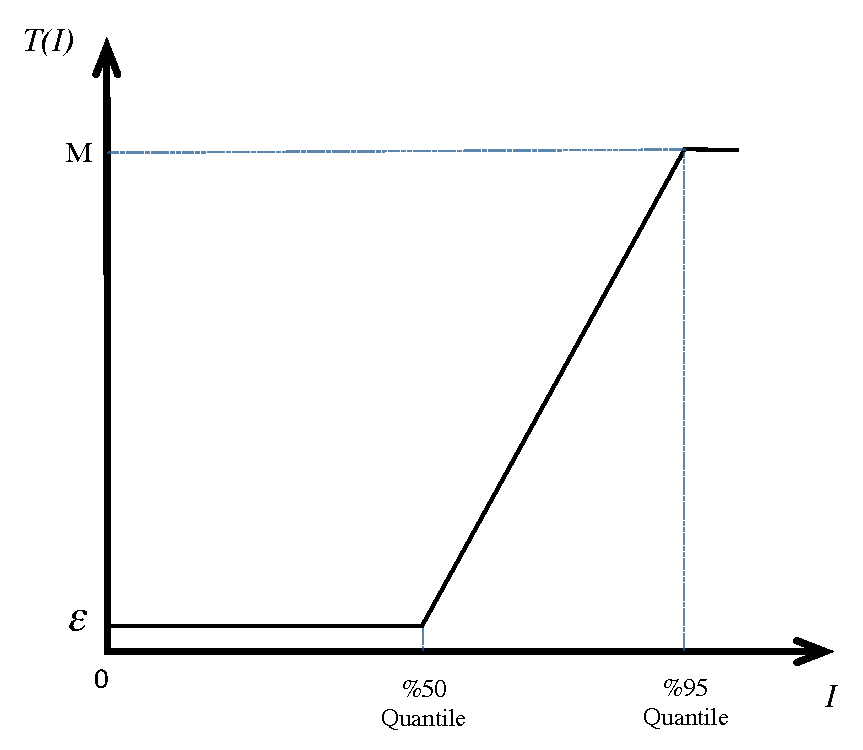
\includegraphics[width=3.45in,height=3in]{IntensityTransFunc}\
\centering
\caption{Intensity transform function. Strong edges (with values above \%95 percentile) are mapped to a maximum value $M$. Weak edges (with values below \%50 percentile) are mapped to a value $\epsilon > 0$ close to zero. Other edges are mapped linearly to a $\epsilon < value < M$.}
\label{IntensityTransFunc}
\end{figure}
%--------------------------------

Once the edge map $\mu$ is estimated, the spatial weights are defined as:

\begin{equation}
\label{eq:spatialWeights}
\begin{gathered}
W(x) = \frac{1}{\mu (x)}
\end{gathered}
\end{equation}

\subsubsection{Experiments and Preliminary Results}
This section presents a series of experiments on a two-dimensional (2D) image data for the initial assessments of the proposed super-resolution reconstruction approach.
The results compared the performance of our SRR method to standard TV and zero-padded IFFT approaches.

\paragraph{Test Data}
Initial assessments were run on two-dimensional data. For this purpose, a sample 3D dataset, listed in Table (\ref{3DSSRTestData}), was selected to create the input 2D test images. This dataset was used as part of the multi-site international PREDICT-HD project and was acquired with a high isotropic ($1 \times 1$ $mm^2$) resolution in the axial plane.

%--------------------------------
\begin{table}[ht]
\centering
\caption{Test dataset for initial assessments}
\label{3DSSRTestData}
\begin{tabular}{|l|l|l|l|l|}
\hline
Scan        & Site                                                            & \begin{tabular}[c]{@{}l@{}}MR \\ vendor\end{tabular} & \begin{tabular}[c]{@{}l@{}}Field \\ strength\end{tabular} & \begin{tabular}[c]{@{}l@{}}Collected \\ modalities\end{tabular}                          \\
\hline \hline
1166\_54860 & 
\begin{tabular}[c]{@{}l@{}}Site\_001\\ (Rochester)\end{tabular} & 
GE Signa HDxt & 
3.0            & 
\begin{tabular}
[c]{@{}l@{}}T1: $1 \times 1 \times 1$ $mm^3$\\ T2: $1 \times 1 \times 1$ $mm^3$\\ DWI: $1 \times 1 \times 2.4$ $mm^3$\end{tabular} \\ 
\hline
\end{tabular}
\end{table}
%--------------------------------

The input baseline and 2D test images were then created as follows. Note that all inputs are aligned in both physical and voxel spaces.

\begin{itemize}
\item[ \textbf{}]{
       \textbf{Baseline 2D DWI image:}
       First, the $b0$ component and the $1^{st}$ gradient component were extracted from the sample 4D diffusion-weighted dataset listed in table (\ref{3DSSRTestData}).
       Then, the mid-axial slice of these components were extracted to serve as our high-resolution ground truth images with the size of $256 \times 256$ and isotropic pixel sizes of $1 \times 1$ $mm^2$.
       }
\item[ \textbf{}]{
       \textbf{Low resolution input DWIs:}
        were created by downsampling the high-resolution baseline images by a factor of $2$ by only keeping the low pass Fourier indices from the high-resolution image.
        }
\item[ \textbf{}]{
       \textbf{Structural MRI input images:}
        were created by extracting the mid-axial slice from the corresponding $T1$/$T2$-weighted images of the same data session.
        }
\end{itemize}

\paragraph{Evaluation Metric}

Signal-to-noise ratio (SNR) was used to compare the output of the proposed SRR method to the results from standard TV and zero-padded IFFT approaches, such that the \textit{higher} SNR value indicates the better reconstruction performance.
For each reconstructed image from the different methods, the SNR was computed as:

\begin{equation}
\label{eq:snr}
\begin{gathered}
SNR = 20\times \log_{10} \frac{\left \| I_0 \right \|_{2}}{\left \| I_{SR} - I_0 \right \|_{2}}
\end{gathered}
\end{equation}

Where $I_{SR}$ is the reconstructed super-resolved DWI image, and $I_0$ is the baseline high-resolution DWI image.

\paragraph{Preliminary 2D results}
Figure (\ref{multimodal_wight_image}) shows the $T1$/$T2$-weighted images, the estimated anatomical edge map, and the created spatial weights based on the method described in section \ref{section:estimateLabelMap}.

%--------------------------------
\begin{figure}
\centering
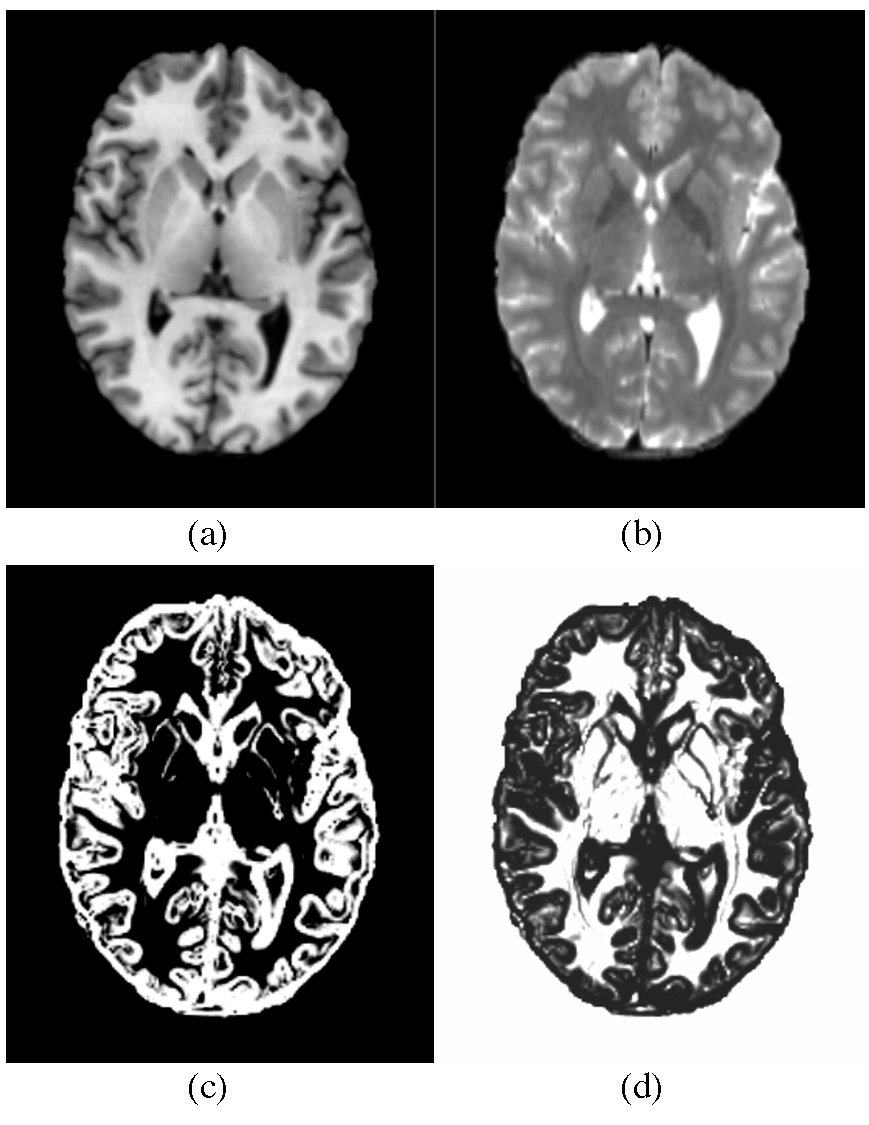
\includegraphics[width=2.9in,height=3.75in]{multimodal_weight_image}\
\centering
\caption{Created spatial weights based on the anatomical edges estimated from the high-resolution structural MR modalities. (a) T1-weighted MR image. (b) T2-weighted MR image. (c) Estimated edge map based on the maximum gradient values as described in section \ref{section:estimateLabelMap}. (d) Prior spatial weights created from estimated edge map based on equation (\ref{eq:spatialWeights}).}
\label{multimodal_wight_image}
\end{figure}
%--------------------------------

The prior spatial weights map was passed to a weighted-TV algorithm along with the input low-resolution 2D test images to create the results of the proposed method.
Proposed approach was tested on both $b0$ and $1^{st}$ gradient components from a 4D DWI dataset.
Figure (\ref{b0_SRR}) shows the performance of our weighted-TV super-resolution reconstruction method compared to standard TV and zero-padded IFFT on a low-resolution $b0$ image.
Figure (\ref{g1_SRR}) shows the same results for the $1^{st}$ gradient component image.

We also provided the reconstruction results using FRI edge map suggest by Jacob and Ongie \cite{ongie2015} demonstrated in Figure (\ref{b0_SRR_FRI}). The FRI method performance is also superior to zero-padded IFFT and standard TV algorithms, and its reconstructed output image is comparable to the results of our proposed method.

%--------------------------------
\begin{figure}[ht]
\centering
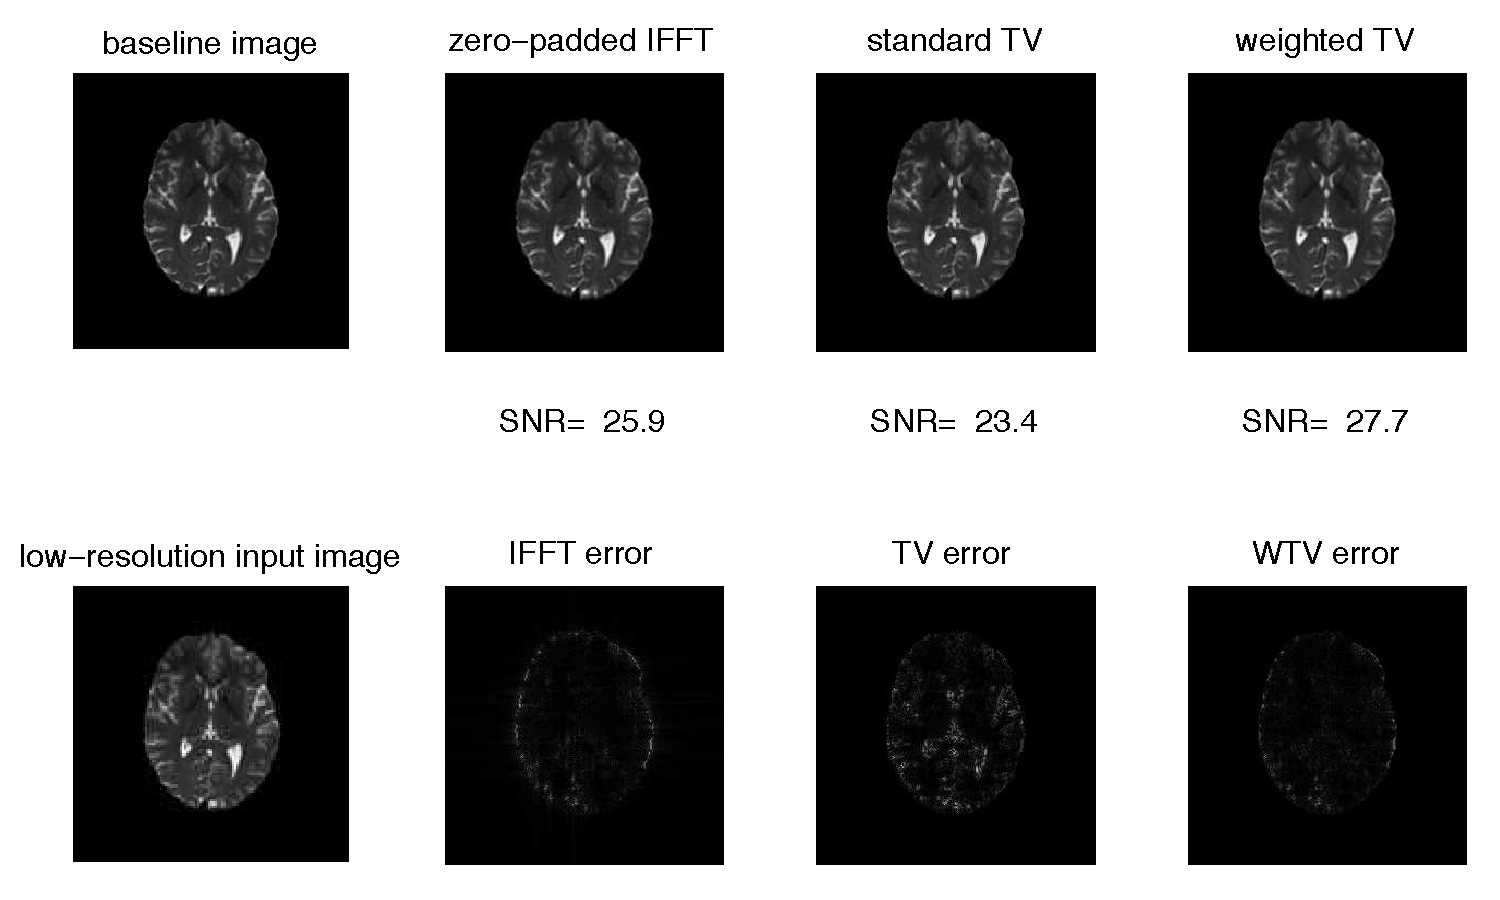
\includegraphics[width=7.5in,height=4.5in]{b0_SRR}\
\centering
\caption{Reconstructed $b_0$ component of a typical DWI subject using $3$ different methods. The SNR value is provided for the result of each method demonstrated in the first row. The second row shows the low-resolution image, by a factor of $2$, and the difference image between each reconstructed image and the original high-resolution baseline image, which is magnified by $20$ times. The higher SNR value for the proposed weighted-TV approach indicates better reconstruction results.}
\label{b0_SRR}
\end{figure}
%--------------------------------

%--------------------------------
\begin{figure}[ht]
\centering
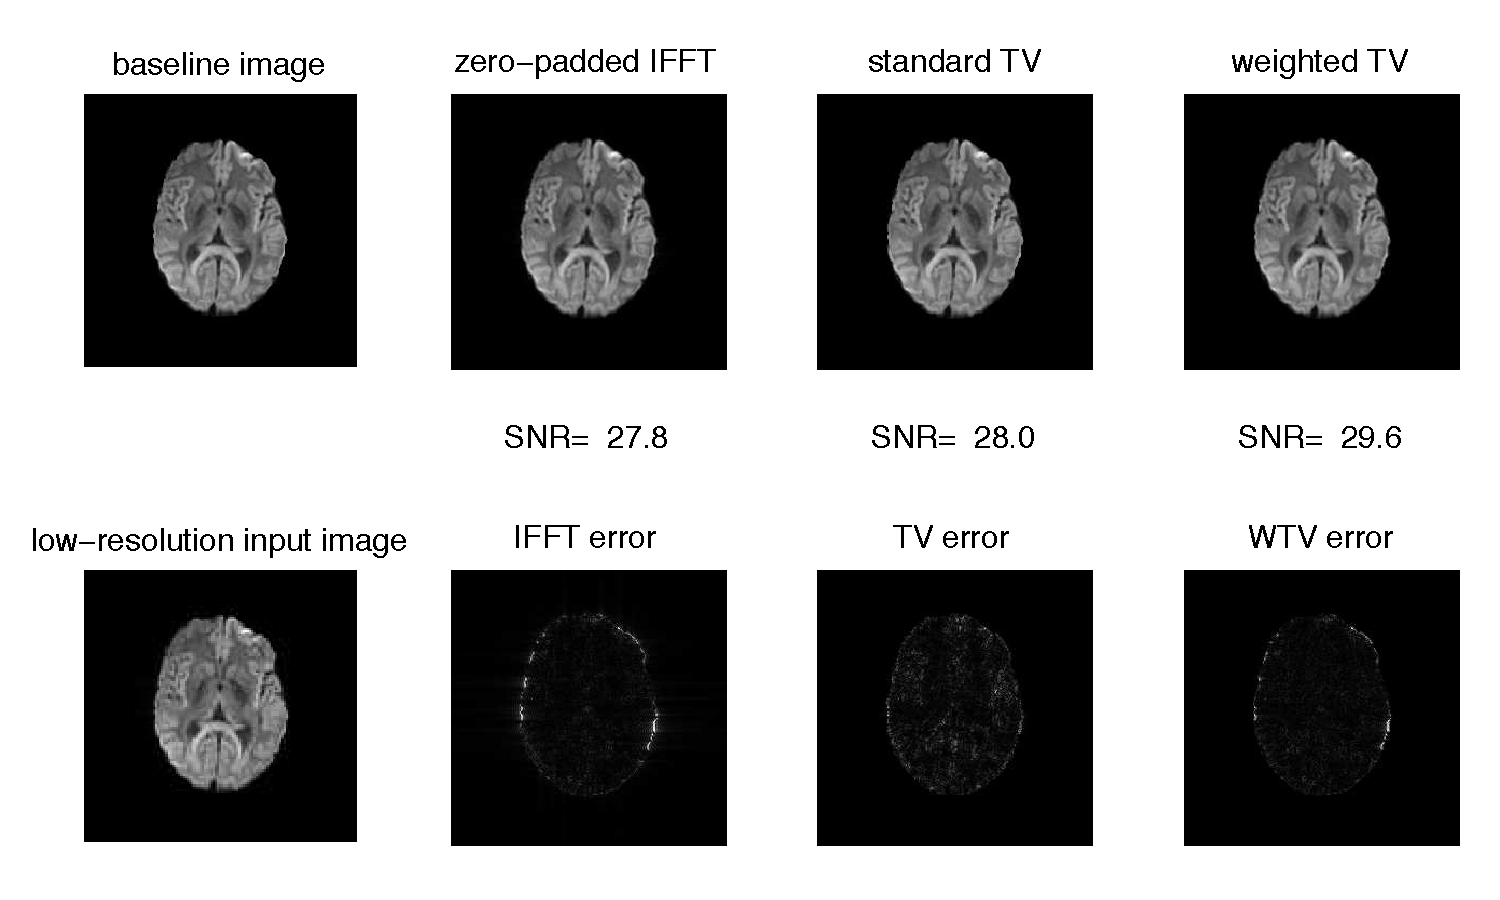
\includegraphics[width=7.5in,height=4.5in]{g1_SRR}\
\centering
\caption{Reconstructed first gradient component of a typical DWI subject using $3$ different methods. The SNR value is provided for the result of each method demonstrated in the first row. The second row shows the low-resolution image, by a factor of $2$, and the difference image between each reconstructed image and the original high-resolution baseline image, which is magnified by $20$ times. The higher SNR value for the proposed weighted-TV approach indicates better reconstruction results for the gradient components as well.}
\label{g1_SRR}
\end{figure}
%--------------------------------

%--------------------------------
\begin{figure}[ht]
\centering
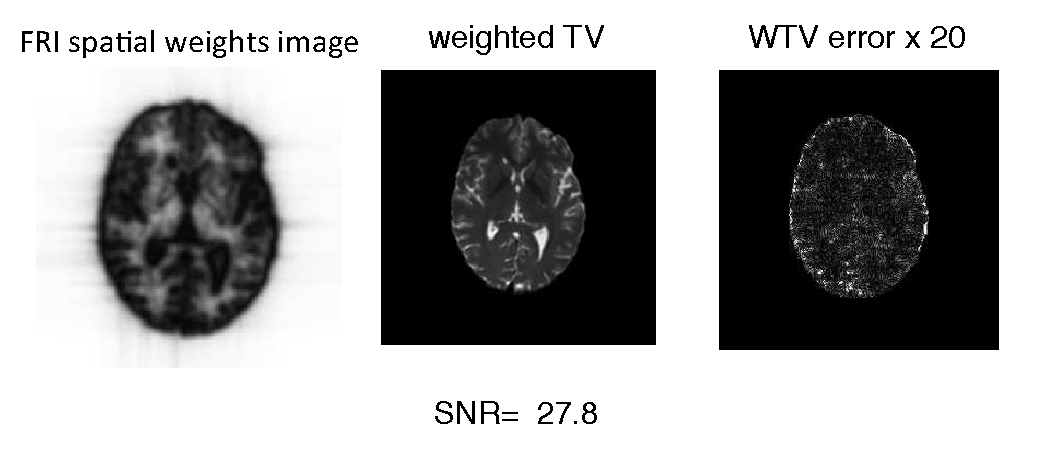
\includegraphics[width=5.25in,height=2.25in]{b0_SRR_FRI}\
\centering
\caption{Reconstructed b0 component of a typical DWI subject using FRI edge map suggest in \cite{ongie2015}.}
\label{b0_SRR_FRI}
\end{figure}
%--------------------------------


\subsubsection{Discussion and conclusions}
The proposed weighted-TV method based on the prior knowledge of the anatomical edges shows superior performance compared to both standard TV and zero-padded IFFT for both $b_0$ and first gradient component.
 
Also, zero-padded IFFT approach gets better results rather than standard TV for the $b_0$ component. The reason is that TV works well for compressed sensing style sampling (when we have sparse samples equally from low and high frequencies) but seems to perform poorly for super-resolution (when mostly higher frequencies are missed). This is specially the case here, since our input real data is a relatively smooth image with no super sharp edges and less high frequency content.

The FRI algorithm has an advantage over our proposed method, since it estimates the anatomical edges from the input low-resolution image, and unlike our method, it does not need complementary information from external sources. However, the proposed approach has following advantages:
\begin{itemize}
\item[-] Using conventional image processing filters makes our method to be easily adoptable for the processing of large-scale multi-site datasets, since there are less parameters needed to be adjusted to work optimally for the analysis of a set of heterogeneous data.
\item[-] Proposed method uses fast conventional image processing tools. It accelerates the process time that can be specially important when the implementation is expanded to operate on real 3D datasets.
\item[-] The introduce FRI algorithm operates in voxel space; however, the proposed method can be easily expanded to operate in physical space, which is important in real world medical imaging applications.
\end{itemize}

\subsubsection{Future Research Study}

\paragraph{Implementation}

Expand the proposed super-resolution reconstruction method to operate on 3D images in physical space.
The software will be implemented based on the Insight Toolkit (ITK) libraries \cite{johnson2015itk1, johnson2015itk2}, such that the implemented framework is applicable on 4D DWI datasets. This software will contribute to a fully automated processing pipeline for MR images.

\paragraph{Evaluation}

The resolution of the routine DWI scans is of $2$ to $3$ $mm$. The goal is to evaluate the performance of the proposed super-resolution reconstruction (SSR) method on this resolution level. 

First, we simulate a group of diffusion-weighted imaging data to have the routine resolution of DWI scans. Then, the recovered results are compared to the ground truth data for quantitative performance evaluation.
The performance of the proposed SRR method will be further compared with the following methods:
\begin{itemize}
\item[-] Nearest neighbor interpolation, Zero-padded IFFT, Standard total variation (TV)
\end{itemize}

\subparagraph{Test Data}
\label{HCPData}

We use a publicly available dataset from WU-Minn \textbf{Human Connectome Project} (HCP) consortium \cite{van2013,sotiropoulos2013}.
The HCP designed $3T$ Siemens Connectome scanner equipped with $100$ $mTm^{-1}$ and $300$ $mTm^{-1}$ gradient coils, that are several times more powerful than standard clinical scanners, and exloited several imaging and image reonstruction innovations to speed up acquisition and improve the data quality \cite{sotiropoulos2013}.

The HCP diffusion-weighted imaging data were acquired with a resolution of $1.25 \times 1.25 \times 1.25$ $mm^3$. 
%High-resolution diffusion-weighted images with resolution of 1.25x1.25x1.25 mm3 were acquired on a 3T Siemens Connectome scanner.
The original HCP data are used as \textit{baselines}.
To simulate a group of typical-resolution DWI as \textit{input sources}, the original HCP data will be downsampled in Fourier domain by a factor of $2$ to obtain DWI with resolution of $2.5 \times 2.5 \times 2.5$ $mm^3$ that is at the similar level of our typical DWI resolution.
\newline

\subparagraph{Experimental methods}

The evaluation experiments need to show whether we meet the goals of this study. Particularly, we are interested in the answers of the following questions:
\begin{itemize}
    \item[-] How can we evaluate the performance of the proposed SRR method using the common approaches used in this literature?
    \item[-] How can we evaluate the effectiveness of our proposed SSR method in providing a better estimate of the brain connectivity and increasing the sensitivity of the scalar measures derived from diffusion data?
    \item[-] How can we evaluate the effectiveness of our proposed SSR method in reducing the partial volume effect?
\end{itemize}

To answer above questions, three different approaches are proposed to evaluate the performance of the proposed SRR method.
The first two experimental methods use the HCP data described in section \ref{HCPData}. The third experimental method will be evaluated on a sample DWI dataset arbitrarily selected from our local University of Iowa
SIEMENS Trio Tim $3$ Tesla scan protocol. This protocol was used as part of the multi-site international PREDICT-HD \cite{PREDICTHD} project.

\subparagraph*{Approach 1}

As a general approach similar to other super-resolution studies \cite{brown2014,shi2015,ongie2015}, the signal-to-noise ratio (SNR), defined in equation (\ref{eq:snr}), will be used as the metric to compare the recovered high-resolution image to the original image.

Higher SNR value will indicate the better reconstruction performance.
This experiment will be run on all $20$ data subjects from HCP, and a paired t-test will be performed in order to compare the quantitative results ($p-value < 0.05$ is considered significant).

\subparagraph*{Approach 2}

A successfully reconstructed high-resolution image presents a better estimate of the underlying anatomical structures, so it can provide a more accurate assessment of the brain connectivity and can improve the clinical practice by increasing the sensitivity of the measures used by clinicians in a neurodegenerative study.
Here we suggest two experiments to evaluate the effectiveness of our proposed SRR approach in providing a better estimate of the brain connectivity and increasing the sensitivity of the scalar measures derived from diffusion data.

In the \textit{first} experiment, tracts of interest will be compared between each recovered high-resolution image and the original image. Following steps are proposed in this regard:
\begin{itemize}
\item[1)] A two-tensor tractography algorithm \cite{Malcolm2010, baumgartner2012} will be run to perform a whole brain tractography.

\item[2)] Cortico-spinal tracts of interest will be extracted using the White Matter Query Language (WMQL), that is a technique to formally describe white matter tracts and to automatically extract them \cite{wassermann2013}.
This query language allows constructing an anatomical definition for each white matter tract including description of the adjacent gray and white matter regions and rules for the spatial relations. Therefore, tracts of interest can be extracted from anatomical knowledge of the human brain white matter.

\item[3)] ``Minimum distance error'' will be used as a metric to compare the shape of the extracted cortico-spinal tracts from each reconstructed image to the shape of the tract extracted from the high-resolution (HR) baseline image.

First, for each point of the tracts in the HR image, we find the closest point in the reconstructed image tracts:

\begin{equation}
\begin{gathered}
\forall p\in \left\{baseline \quad image \quad tracts \right\}, \\
%\forall p\in \text{$\{$ baseline image tract $\}$}, \\
\forall q\in \left\{reconstructed \quad image \quad tracts \right\}, \\
%\forall q\in \text{$\{$ reconstructed image tract $\}$}, \\
\quad \exists \quad \hat{q} \quad s.t. \quad
\hat{q} = arg\min_q(\left \| p - q \right \|)
\end{gathered}
\end{equation}

Then, a mean square error is calculated over all points $p$ and their computed corresponding closest points:

\begin{equation}
\label{eq:minDist}
\begin{gathered}
\text{Minimum Distance Error} = \sum_{p} \left \| p - \hat{q} \right \|^2
\end{gathered}
\end{equation}

Lower ``minimum distance error'' indicates better performance, since it indicates more similarity between the tracts shape in the baseline image and each output reconstructed image.

\end{itemize}

Rotationally invariant scalars (RISs) are numeric representations
of diffusion shape and magnitude. They are important measures for clinicians and are useful biomarkers of disease progression.
Computing the average of Fractional Anisotropy (FA) inside the important anatomical regions is another way to evaluate the performance of different SSR methods in increasing the sensitivity of scalar measures.

In the \textit{second} experiment, the average of FA is measured for all points $p$ in the extracted cortico-spinal tracts of the HR baseline image, and this measure will be compared between all reconstructed high-resolution images:

\begin{equation}
\label{eq:avgFA}
\begin{gathered}
\text{Difference FA Average} = \frac{1}{N_p}\sum_{p} (FA_i(p) - FA_b(p))
\end{gathered}
\end{equation}

Where $N_p$ is the number of points in the cortico-spinal tracts extracted from HR baseline image. 
$FA_i(p)$ is the FA value at point $p$ computed from the $i_{th}$ output reconstructed image, and $FA_b(p)$ is the FA value at point $p$ computed from high-resolution baseline image.
Lower ``Difference FA Average'' indicates better performance.

Both of above experimental methods will be run on all $20$ data subjects from HCP, and a paired t-test will be performed in order to compare the quantitative results ($p-value < 0.05$ is considered significant).

\subparagraph*{Approach 3}

High-resolution images are critical to reduce the partial volume effects (PVE). In the last experimental approach, we compare the performance of different SRR methods in reducing the PVE in an important anatomical white matter region.

First, the pure plugs mask, generated in Aim 1, will be used to identify all the pures and mixed samples inside the region of interest.
For a single tissue region, we expect that the average of FA computed within only pure plugs be approximately the same before and after super-resolution reconstruction. This value can be used as the gold standard measure for this experimental method.

Then, the average FA is computed within only non-pure plugs inside the region of interest, and this measure will be compared to the baseline measure before and after super-resolution reconstruction by each SSR methods.

This approach will be performed on a $b0$ component from a sample DWI dataset, as listed in Table (\ref{PurePlugsMaskTestData}), which is arbitrary selected from our local University of Iowa SIEMENS Trio Tim $3$ Tesla scan protocol.
\newline

\subsubsection{Expected Results}

As suggested by preliminary $2D$ results, demonstrated by Figures (\ref{b0_SRR}, \ref{g1_SRR}), we expect that the proposed method outperforms the other SRR approaches when it is evaluated on $4D$ DWI datasets.

We expect that the proposed method leads to better clinical practices by increasing the sensitivity of the scalar measures used as disease progression biomarkers as described in section \ref{clinicalBackground}.
\newline

\subsubsection{Potential Problems}

To apply the proposed method on a $4D$ DWI dataset, the weighted-TV minimization algorithm needs to be run for each $b_0$ and gradient component in a DWI dataset. Since our typical DWI dataset includes $82$ volume components, the current implementation may perform too slow in a real world application. In this case, we should investigate different developed optimization methods in the literature \cite{marquina2008, zhu2008, chambolle2011} and use the most efficient approach to solve the minimization problem in equation (\ref{eq:weightedregularization}).
\newline

\subsubsection{Status}
\begin{itemize}
    \item The proposed super-resolution reconstruction method has been developed in $2D$ voxel space, and the initial assessments have been run on a sample dataset from PREDICT-HD study.
    \item The expansion of the proposed method to operate in physical $3D$ space is under development.
    \item The proposed method needs to be evaluated on $4D$ DWI datasets using the the proposed experimental approaches.
    \item The proposed method and the evaluation results will be submitted as a paper to frontiers in neuroscience journal or IEEE transactions on biomedical engineering.
\end{itemize}









\clearpage